%%%%%%%%%%%%%%%%%%%%%%%%%%%%%%%%%%%%%%%%%%%%%%%%%%%%%%%%%%%%%%%%%%%%%%
% Template for a UBC-compliant dissertation
% At the minimum, you will need to change the information found
% after the "Document meta-data"
%
%!TEX TS-program = pdflatex
%!TEX encoding = UTF-8 Unicode

%% The ubcdiss class provides several options:
%%   gpscopy (aka fogscopy)
%%       set parameters to exactly how GPS specifies
%%         * single-sided
%%         * page-numbering starts from title page
%%         * the lists of figures and tables have each entry prefixed
%%           with 'Figure' or 'Table'
%%       This can be tested by `\ifgpscopy ... \else ... \fi'
%%   10pt, 11pt, 12pt
%%       set default font size
%%   oneside, twoside
%%       whether to format for single-sided or double-sided printing
%%   balanced
%%       when double-sided, ensure page content is centred
%%       rather than slightly offset (the default)
%%   singlespacing, onehalfspacing, doublespacing
%%       set default inter-line text spacing; the ubcdiss class
%%       provides \textspacing to revert to this configured spacing
%%   draft
%%       disable more intensive processing, such as including
%%       graphics, etc.
%%

% For submission to GPS
\documentclass[gpscopy,onehalfspacing,11pt]{ubcdiss}

% For your own copies (looks nicer)
% \documentclass[balanced,twoside,11pt]{ubcdiss}

%%%%%%%%%%%%%%%%%%%%%%%%%%%%%%%%%%%%%%%%%%%%%%%%%%%%%%%%%%%%%%%%%%%%%%
%%%%%%%%%%%%%%%%%%%%%%%%%%%%%%%%%%%%%%%%%%%%%%%%%%%%%%%%%%%%%%%%%%%%%%
%%
%% FONTS:
%% 
%% The defaults below configures Times Roman for the serif font,
%% Helvetica for the sans serif font, and Courier for the
%% typewriter-style font.  Configuring fonts can be time
%% consuming; we recommend skipping to END FONTS!
%% 
%% If you're feeling brave, have lots of time, and wish to use one
%% your platform's native fonts, see the commented out bits below for
%% XeTeX/XeLaTeX.  This is not for the faint at heart. 
%% (And shouldn't you be writing? :-)
%%

%% NFSS font specification (New Font Selection Scheme)
\usepackage{times,mathptmx,courier}
\usepackage[scaled=.92]{helvet}

%% Math or theory people may want to include the handy AMS macros
%\usepackage{amssymb}
%\usepackage{amsmath}
%\usepackage{amsfonts}

%% The pifont package provides access to the elements in the dingbat font.   
%% Use \ding{##} for a particular dingbat (see p7 of psnfss2e.pdf)
%%   Useful:
%%     51,52 different forms of a checkmark
%%     54,55,56 different forms of a cross (saltyre)
%%     172-181 are 1-10 in open circle (serif)
%%     182-191 are 1-10 black circle (serif)
%%     192-201 are 1-10 in open circle (sans serif)
%%     202-211 are 1-10 in black circle (sans serif)
%% \begin{dinglist}{##}\item... or dingautolist (which auto-increments)
%% to create a bullet list with the provided character.
\usepackage{pifont}

%%%%%%%%%%%%%%%%%%%%%%%%%%%%%%%%%%%%%%%%%%%%%%%%%%%%%%%%%%%%%%%%%%%%%%
%% Configure fonts for XeTeX / XeLaTeX using the fontspec package.
%% Be sure to check out the fontspec documentation.
%\usepackage{fontspec,xltxtra,xunicode}	% required
%\defaultfontfeatures{Mapping=tex-text}	% recommended
%% Minion Pro and Myriad Pro are shipped with some versions of
%% Adobe Reader.  Adobe representatives have commented that these
%% fonts can be used outside of Adobe Reader.
%\setromanfont[Numbers=OldStyle]{Minion Pro}
%\setsansfont[Numbers=OldStyle,Scale=MatchLowercase]{Myriad Pro}
%\setmonofont[Scale=MatchLowercase]{Andale Mono}

%% Other alternatives:
%\setromanfont[Mapping=tex-text]{Adobe Caslon}
%\setsansfont[Scale=MatchLowercase]{Gill Sans}
%\setsansfont[Scale=MatchLowercase,Mapping=tex-text]{Futura}
%\setmonofont[Scale=MatchLowercase]{Andale Mono}
%\newfontfamily{\SYM}[Scale=0.9]{Zapf Dingbats}
%% END FONTS
%%%%%%%%%%%%%%%%%%%%%%%%%%%%%%%%%%%%%%%%%%%%%%%%%%%%%%%%%%%%%%%%%%%%%%
%%%%%%%%%%%%%%%%%%%%%%%%%%%%%%%%%%%%%%%%%%%%%%%%%%%%%%%%%%%%%%%%%%%%%%



%%%%%%%%%%%%%%%%%%%%%%%%%%%%%%%%%%%%%%%%%%%%%%%%%%%%%%%%%%%%%%%%%%%%%%
%%%%%%%%%%%%%%%%%%%%%%%%%%%%%%%%%%%%%%%%%%%%%%%%%%%%%%%%%%%%%%%%%%%%%%
%%
%% Recommended packages
%%
\usepackage{checkend}	% better error messages on left-open environments
\usepackage{graphicx}	% for incorporating external images

%% booktabs: provides some special commands for typesetting tables as used
%% in excellent journals.  Ignore the examples in the Lamport book!
\usepackage{booktabs}

%% listings: useful support for including source code listings, with
%% optional special keyword formatting.  The \lstset{} causes
%% the text to be typeset in a smaller sans serif font, with
%% proportional spacing.
\usepackage{listings}
\lstset{basicstyle=\sffamily\scriptsize,showstringspaces=false,fontadjust}

%% The acronym package provides support for defining acronyms, providing
%% their expansion when first used, and building glossaries.  See the
%% example in glossary.tex and the example usage throughout the example
%% document.
%% NOTE: to use \MakeTextLowercase in the \acsfont command below,
%%   we *must* use the `nohyperlinks' option -- it causes errors with
%%   hyperref otherwise.  See Section 5.2 in the ``LaTeX 2e for Class
%%   and Package Writers Guide'' (clsguide.pdf) for details.
\usepackage[printonlyused,nohyperlinks]{acronym}
%% The ubcdiss.cls loads the `textcase' package which provides commands
%% for upper-casing and lower-casing text.  The following causes
%% the acronym package to typeset acronyms in small-caps
%% as recommended by Bringhurst.
\renewcommand{\acsfont}[1]{{\scshape \MakeTextLowercase{#1}}}

%% color: add support for expressing colour models.  Grey can be used
%% to great effect to emphasize other parts of a graphic or text.
%% For an excellent set of examples, see Tufte's "Visual Display of
%% Quantitative Information" or "Envisioning Information".
\usepackage{color}
\definecolor{greytext}{gray}{0.5}

%% comment: provides a new {comment} environment: all text inside the
%% environment is ignored.
%%   \begin{comment} ignored text ... \end{comment}
\usepackage{comment}

%% The natbib package provides more sophisticated citing commands
%% such as \citeauthor{} to provide the author names of a work,
%% \citet{} to produce an author-and-reference citation,
%% \citep{} to produce a parenthetical citation.
%% We use \citeeg{} to provide examples
\usepackage[numbers,sort&compress]{natbib}
\newcommand{\citeeg}[1]{\citep[e.g.,][]{#1}}

%% The titlesec package provides commands to vary how chapter and
%% section titles are typeset.  The following uses more compact
%% spacings above and below the title.  The titleformat that follow
%% ensure chapter/section titles are set in singlespace.
\usepackage[compact]{titlesec}
\titleformat*{\section}{\singlespacing\raggedright\bfseries\Large}
\titleformat*{\subsection}{\singlespacing\raggedright\bfseries\large}
\titleformat*{\subsubsection}{\singlespacing\raggedright\bfseries}
\titleformat*{\paragraph}{\singlespacing\raggedright\itshape}

%% The caption package provides support for varying how table and
%% figure captions are typeset.
\usepackage[format=hang,indention=-1cm,labelfont={bf},margin=1em]{caption}

%% url: for typesetting URLs and smart(er) hyphenation.
%% \url{http://...} 
\usepackage{url}
\urlstyle{sf}	% typeset urls in sans-serif


%%%%%%%%%%%%%%%%%%%%%%%%%%%%%%%%%%%%%%%%%%%%%%%%%%%%%%%%%%%%%%%%%%%%%%
%%%%%%%%%%%%%%%%%%%%%%%%%%%%%%%%%%%%%%%%%%%%%%%%%%%%%%%%%%%%%%%%%%%%%%
%%
%% Possibly useful packages: you may need to explicitly install
%% these from CTAN if they aren't part of your distribution;
%% teTeX seems to ship with a smaller base than MikTeX and MacTeX.
%%
%\usepackage{pdfpages}	% insert pages from other PDF files
%\usepackage{longtable}	% provide tables spanning multiple pages
%\usepackage{chngpage}	% support changing the page widths on demand
%\usepackage{tabularx}	% an enhanced tabular environment

%% enumitem: support pausing and resuming enumerate environments.
%\usepackage{enumitem}

%% rotating: provides two environments, sidewaystable and sidewaysfigure,
%% for typesetting tables and figures in landscape mode.  
%\usepackage{rotating}

%% subfig: provides for including subfigures within a figure,
%% and includes being able to separately reference the subfigures.
%\usepackage{subfig}

%% ragged2e: provides several new new commands \Centering, \RaggedLeft,
%% \RaggedRight and \justifying and new environments Center, FlushLeft,
%% FlushRight and justify, which set ragged text and are easily
%% configurable to allow hyphenation.
%\usepackage{ragged2e}

%% The ulem package provides a \sout{} for striking out text and
%% \xout for crossing out text.  The normalem and normalbf are
%% necessary as the package messes with the emphasis and bold fonts
%% otherwise.
%\usepackage[normalem,normalbf]{ulem}    % for \sout

%%%%%%%%%%%%%%%%%%%%%%%%%%%%%%%%%%%%%%%%%%%%%%%%%%%%%%%%%%%%%%%%%%%%%%
%% HYPERREF:
%% The hyperref package provides for embedding hyperlinks into your
%% document.  By default the table of contents, references, citations,
%% and footnotes are hyperlinked.
%%
%% Hyperref provides a very handy command for doing cross-references:
%% \autoref{}.  This is similar to \ref{} and \pageref{} except that
%% it automagically puts in the *type* of reference.  For example,
%% referencing a figure's label will put the text `Figure 3.4'.
%% And the text will be hyperlinked to the appropriate place in the
%% document.
%%
%% Generally hyperref should appear after most other packages

%% The following puts hyperlinks in very faint grey boxes.
%% The `pagebackref' causes the references in the bibliography to have
%% back-references to the citing page; `backref' puts the citing section
%% number.  See further below for other examples of using hyperref.
%% 2009/12/09: now use `linktocpage' (Jacek Kisynski): GPS now prefers
%%   that the ToC, LoF, LoT place the hyperlink on the page number,
%%   rather than the entry text.
\usepackage[bookmarks,bookmarksnumbered,%
    allbordercolors={0.8 0.8 0.8},%
    pagebackref,linktocpage%
    ]{hyperref}
%% The following change how the the back-references text is typeset in a
%% bibliography when `backref' or `pagebackref' are used
%%
%% Change \nocitations if you'd like some text shown where there
%% are no citations found (e.g., pulled in with \nocite{xxx})
\newcommand{\nocitations}{\relax}
%%\newcommand{\nocitations}{No citations}
%%
%\renewcommand*{\backref}[1]{}% necessary for backref < 1.33
\renewcommand*{\backrefsep}{,~}%
\renewcommand*{\backreftwosep}{,~}% ', and~'
\renewcommand*{\backreflastsep}{,~}% ' and~'
\renewcommand*{\backrefalt}[4]{%
\textcolor{greytext}{\ifcase #1%
\nocitations%
\or
\(\rightarrow\) page #2%
\else
\(\rightarrow\) pages #2%
\fi}}


%% The following uses most defaults, which causes hyperlinks to be
%% surrounded by colourful boxes; the colours are only visible in
%% PDFs and don't show up when printed:
%\usepackage[bookmarks,bookmarksnumbered]{hyperref}

%% The following disables the colourful boxes around hyperlinks.
%\usepackage[bookmarks,bookmarksnumbered,pdfborder={0 0 0}]{hyperref}

%% The following disables all hyperlinking, but still enabled use of
%% \autoref{}
%\usepackage[draft]{hyperref}

%% The following commands causes chapter and section references to
%% uppercase the part name.
\renewcommand{\chapterautorefname}{Chapter}
\renewcommand{\sectionautorefname}{Section}
\renewcommand{\subsectionautorefname}{Section}
\renewcommand{\subsubsectionautorefname}{Section}

%% If you have long page numbers (e.g., roman numbers in the 
%% preliminary pages for page 28 = xxviii), you might need to
%% uncomment the following and tweak the \@pnumwidth length
%% (default: 1.55em).  See the tocloft documentation at
%% http://www.ctan.org/tex-archive/macros/latex/contrib/tocloft/
% \makeatletter
% \renewcommand{\@pnumwidth}{3em}
% \makeatother

%%%%%%%%%%%%%%%%%%%%%%%%%%%%%%%%%%%%%%%%%%%%%%%%%%%%%%%%%%%%%%%%%%%%%%
%%%%%%%%%%%%%%%%%%%%%%%%%%%%%%%%%%%%%%%%%%%%%%%%%%%%%%%%%%%%%%%%%%%%%%
%%
%% Some special settings that controls how text is typeset
%%
% \raggedbottom		% pages don't have to line up nicely on the last line
% \sloppy		% be a bit more relaxed in inter-word spacing
% \clubpenalty=10000	% try harder to avoid orphans
% \widowpenalty=10000	% try harder to avoid widows
% \tolerance=1000

%% And include some of our own useful macros
% This file provides examples of some useful macros for typesetting
% dissertations.  None of the macros defined here are necessary beyond
% for the template documentation, so feel free to change, remove, and add
% your own definitions.
%
% We recommend that you define macros to separate the semantics
% of the things you write from how they are presented.  For example,
% you'll see definitions below for a macro \file{}: by using
% \file{} consistently in the text, we can change how filenames
% are typeset simply by changing the definition of \file{} in
% this file.
% 
%% The following is a directive for TeXShop to indicate the main file
%%!TEX root = diss.tex

\newcommand{\NA}{\textsc{n/a}}	% for "not applicable"
\newcommand{\eg}{e.g.,\ }	% proper form of examples (\eg a, b, c)
\newcommand{\ie}{i.e.,\ }	% proper form for that is (\ie a, b, c)
\newcommand{\etal}{\emph{et al}}

% Some useful macros for typesetting terms.
\newcommand{\file}[1]{\texttt{#1}}
\newcommand{\class}[1]{\texttt{#1}}
\newcommand{\latexpackage}[1]{\href{http://www.ctan.org/macros/latex/contrib/#1}{\texttt{#1}}}
\newcommand{\latexmiscpackage}[1]{\href{http://www.ctan.org/macros/latex/contrib/misc/#1.sty}{\texttt{#1}}}
\newcommand{\env}[1]{\texttt{#1}}
\newcommand{\BibTeX}{Bib\TeX}

% Define a command \doi{} to typeset a digital object identifier (DOI).
% Note: if the following definition raise an error, then you likely
% have an ancient version of url.sty.  Either find a more recent version
% (3.1 or later work fine) and simply copy it into this directory,  or
% comment out the following two lines and uncomment the third.
\DeclareUrlCommand\DOI{}
\newcommand{\doi}[1]{\href{http://dx.doi.org/#1}{\DOI{doi:#1}}}
%\newcommand{\doi}[1]{\href{http://dx.doi.org/#1}{doi:#1}}

% Useful macro to reference an online document with a hyperlink
% as well with the URL explicitly listed in a footnote
% #1: the URL
% #2: the anchoring text
\newcommand{\webref}[2]{\href{#1}{#2}\footnote{\url{#1}}}

% epigraph is a nice environment for typesetting quotations
\makeatletter
\newenvironment{epigraph}{%
	\begin{flushright}
	\begin{minipage}{\columnwidth-0.75in}
	\begin{flushright}
	\@ifundefined{singlespacing}{}{\singlespacing}%
    }{
	\end{flushright}
	\end{minipage}
	\end{flushright}}
\makeatother

% \FIXME{} is a useful macro for noting things needing to be changed.
% The following definition will also output a warning to the console
\newcommand{\FIXME}[1]{\typeout{**FIXME** #1}\textbf{[FIXME: #1]}}

% END


%%%%%%%%%%%%%%%%%%%%%%%%%%%%%%%%%%%%%%%%%%%%%%%%%%%%%%%%%%%%%%%%%%%%%%
%%%%%%%%%%%%%%%%%%%%%%%%%%%%%%%%%%%%%%%%%%%%%%%%%%%%%%%%%%%%%%%%%%%%%%
%%
%% Document meta-data: be sure to also change the \hypersetup information
%%

\title{Investigating the impact of Normalizing flows on Latent Variable Machine Translation}
%\subtitle{If you want a subtitle}

\author{Michael Przystupa}
\previousdegree{Bachelors of Science, University of British Columbia, 2017}
%\previousdegree{M. Silly Walks, Another University, 1994}

% What is this dissertation for?
\degreetitle{Master's Thesis}

\institution{The University of British Columbia}
\campus{Vancouver}

\faculty{FACULTY OF GRADUATE AND POSTDOCTORAL STUDIES}
\department{Computer Science}
\submissionmonth{August}
\submissionyear{2019}

% details of your examining committee
\examiningcommittee{Muhammad Abdul-Mageed, Information Sciences}{Supervisor}
\examiningcommittee{Mark Schmidt, Computer Science}%
    {Supervisor}
%\examiningcommittee{Nebulous Name, Department}{Supervisory Committee Member}

% details of your supervisory committee
\supervisorycommittee{Leonid Sigal, Computer Science}%
    {Supervisory Committee Member}
%\supervisorycommittee{Adeline Long, \textsc{CEO} of Aerial Machine
 %   Transportation, Inc.}{Supervisory Committee Member}

%% hyperref package provides support for embedding meta-data in .PDF
%% files
\hypersetup{
  pdftitle={Change this title!  (DRAFT: \today)},
  pdfauthor={Johnny Canuck},
  pdfkeywords={Your keywords here}
}

%%%%%%%%%%%%%%%%%%%%%%%%%%%%%%%%%%%%%%%%%%%%%%%%%%%%%%%%%%%%%%%%%%%%%%
%%%%%%%%%%%%%%%%%%%%%%%%%%%%%%%%%%%%%%%%%%%%%%%%%%%%%%%%%%%%%%%%%%%%%%
%% 
%% The document content
%%

%% LaTeX's \includeonly commands causes any uses of \include{} to only
%% include files that are in the list.  This is helpful to produce
%% subsets of your thesis (e.g., for committee members who want to see
%% the dissertation chapter by chapter).  It also saves time by 
%% avoiding reprocessing the entire file.
%\includeonly{intro,conclusions}
%\includeonly{discussion}



\usepackage{microtype}
\usepackage{graphicx}
%\usepackage{subfigure}
\usepackage{booktabs} % for professional tables
\usepackage{amsmath}
\usepackage{amssymb}


%Michael defined stuff
\newcommand\reminder[1]{\textcolor{magenta}{ #1}}
\def\cond{\; | \;} 
\DeclareMathOperator{\E}{\mathbb{E}}

\begin{document}

%%%%%%%%%%%%%%%%%%%%%%%%%%%%%%%%%%%%%%%%%%%%%%%%%%
%% From Thesis Components: Tradtional Thesis
%% <http://www.grad.ubc.ca/current-students/dissertation-thesis-preparation/order-components>

% Preliminary Pages (numbered in lower case Roman numerals)
%    1. Title page (mandatory)
\maketitle

%    2. Committee page (mandatory): lists supervisory committee and,
%    if applicable, the examining committee
\makecommitteepage

%    3. Abstract (mandatory - maximum 350 words)
%% The following is a directive for TeXShop to indicate the main file
%%!TEX root = diss.tex

\chapter{Abstract}

Incorporating latent variables in neural machine translation systems allows explicit representations for lexical and semantic information. These representations help improve general translation quality, as well as provide more robust longer sentence and out-of-domain translations. Previous work has focused on using variational inference with isotropic Gaussian distributions, which we hypothesize cannot sufficiently encode latent factors of language which could exhibit multi-modal distributive behavior. Normalizing flows are an approach that enable more flexible posterior distribution estimates by introduce a change of variables with invertible functions. They have previously been applied successfully in computer vision to enable more flexible posterior distributions of image data. In this work, we add normalizing flows on top of two previously proposed methods for latent variable machine translation and compare model performances with and without normalizing flows with changes to the model configuration. We also look at the impact of including latent variables in general when evaluated with the BLEU score.  \reminder{Update what is done when...it's done} %we present our preliminary results for the effects normalizing flows can have on existing latent variable neural machine translation models as a means to improve translation quality. 


% Consider placing version information if you circulate multiple drafts
%\vfill
%\begin{center}
%\begin{sf}
%\fbox{Revision: \today}
%\end{sf}
%\end{center}

\cleardoublepage

%    4. Lay Summary (Effective May 2017, mandatory - maximum 150 words)
%% The following is a directive for TeXShop to indicate the main file
%%!TEX root = diss.tex

%% https://www.grad.ubc.ca/current-students/dissertation-thesis-preparation/preliminary-pages
%% 
%% LAY SUMMARY Effective May 2017, all theses and dissertations must
%% include a lay summary.  The lay or public summary explains the key
%% goals and contributions of the research/scholarly work in terms that
%% can be understood by the general public. It must not exceed 150
%% words in length.

\chapter{Lay Summary}

The lay or public summary explains the key goals and contributions of
the research\slash{}scholarly work in terms that can be understood by the
general public. It must not exceed 150 words in length.

\cleardoublepage

%    5. Preface
%% The following is a directive for TeXShop to indicate the main file
%%!TEX root = diss.tex

\chapter{Preface}

At \ac{UBC}, a preface may be required.  Be sure to check the
\ac{GPS} guidelines as they may have specific content to be included.

\cleardoublepage

%    6. Table of contents (mandatory - list all items in the preliminary pages
%    starting with the abstract, followed by chapter headings and
%    subheadings, bibliographies and appendices)
\tableofcontents
\cleardoublepage	% required by tocloft package

%    7. List of tables (mandatory if thesis has tables)
\listoftables
\cleardoublepage	% required by tocloft package

%    8. List of figures (mandatory if thesis has figures)
\listoffigures
\cleardoublepage	% required by tocloft package

%    9. List of illustrations (mandatory if thesis has illustrations)
%   10. Lists of symbols, abbreviations or other (optional)

%   11. Glossary (optional)
%% The following is a directive for TeXShop to indicate the main file
%%!TEX root = diss.tex

\chapter{Glossary}

%This glossary uses the handy \latexpackage{acroynym} package to automatically
%maintain the glossary.  It uses the package's \texttt{printonlyused}
%option to include only those acronyms explicitly referenced in the
%\LaTeX\ source.

% use \acrodef to define an acronym, but no listing
%\acrodef{UI}{user interface}
%\acrodef{UBC}{University of British Columbia}

% The acronym environment will typeset only those acronyms that were
% *actually used* in the course of the document
\begin{acronym}[ANOVA]
	\acro{NLP}{Natural Language Process}
	\acro{VAE}{variational autoencoder}
	\acro{NMT}{neural machine translation}
	\acro{LVNMT}{latent variable neural machine translation}
	\acro{ELBO}{Evidence Lower Bound}
	\acro{RNN}{recurrent neural network}
	\acro{SOTA}{state of the art}
	\acro{seq2seq}{sequence to sequence}
	\acro{MLP}{multi-layer perceptron}
	
\end{acronym}

%\begin{acronym}
%\acro{ANOVA}[ANOVA]{Analysis of Variance\acroextra{, a set of
%		statistical techniques to identify sources of variability between groups}}
%\acro{API}{application programming interface}
%\acro{CTAN}{\acroextra{The }Common \TeX\ Archive Network}
%\acro{DOI}{Document Object Identifier\acroextra{ (see \url{http://doi.org})}}
%\acro{GPS}[GPS]{Graduate and Postdoctoral Studies}
%\acro{PDF}{Portable Document Format}
%\acro{RCS}[RCS]{Revision control system\acroextra{, a software tool for tracking changes to a set of files}}
%\acro{TLX}[TLX]{Task Load Index\acroextra{, an instrument for gauging the subjective mental workload experienced by a human in performing a task}}
%\acro{UML}{Unified Modelling Language\acroextra{, a visual language for modelling the structure of software artefacts}}
%\acro{URL}{Unique Resource Locator\acroextra{, used to describe a
%    means for obtaining some resource on the world wide web}}
%\acro{W3C}[W3C]{\acroextra{the }World Wide Web Consortium\acroextra{,the standards body for web technologies}}
%\acro{XML}{Extensible Markup Language}
%\end{acronym}

% You can also use \newacro{}{} to only define acronyms
% but without explictly creating a glossary
% 
% \newacro{ANOVA}[ANOVA]{Analysis of Variance\acroextra{, a set of
%   statistical techniques to identify sources of variability between groups.}}
% \newacro{API}[API]{application programming interface}
% \newacro{GOMS}[GOMS]{Goals, Operators, Methods, and Selection\acroextra{,
%   a framework for usability analysis.}}
% \newacro{TLX}[TLX]{Task Load Index\acroextra{, an instrument for gauging
%   the subjective mental workload experienced by a human in performing
%   a task.}}
% \newacro{UI}[UI]{user interface}
% \newacro{UML}[UML]{Unified Modelling Language}
% \newacro{W3C}[W3C]{World Wide Web Consortium}
% \newacro{XML}[XML]{Extensible Markup Language}
	% always input, since other macros may rely on it

\textspacing		% begin one-half or double spacing

%   12. Acknowledgements (optional)
%% The following is a directive for TeXShop to indicate the main file
%%!TEX root = diss.tex

\chapter{Acknowledgements}

%Thank those people who helped you. 

%Don't forget your parents or loved ones.

%You may wish to acknowledge your funding sources.

Thank you to my supervisors Muhammad Abdul-Mageed and Mark Schmidt for their support throughout this whole project. Thank you to Frank Wood for several informative discussions on focusing on  latent variable models for machine translation. Thank you to William Harvey who helped with understanding the \textit{Pyro} probabilistic programming language in which all models were implemented. Thank you to my parents who have loved and supported me through the years, and to my sister who helped improve my writing over the years. Thank you to the University of British Columbia for all the memories. 

%   13. Dedication (optional)

% Body of Thesis (not all sections may apply)
\mainmatter

\acresetall	% reset all acronyms used so far

%    1. Introduction
%% The following is a directive for TeXShop to indicate the main file
%%!TEX root = diss.tex

\chapter{Introduction}
\label{ch:Introduction}

%\section{Introduction}
Incorporating latent variables to explicitly capture aspects of language, such as semantics, has previously been shown to improve \ac{NMT} quality. This includes difficult scenarios in machine translation, such as translating longer sentences better \cite{Zhang2016VNMT, harshil2018GNMT, Su2018VRNMT}, demonstrating robustness to domain mis-match between training and test data \cite{eikema2018AEVNMT}, as well as enabling word level imputation for noisy sentences \cite{harshil2018GNMT}. 

Another utility of \ac{LVNMT} systems is encoding lexical variation. This is achieved by sampling from the latent variables and using beam search to find semantically similar sentences \cite{schulz2018StochasticDecoder, shen2019diverse}. Generating semantically meaningful sentences is a useful property, because research has shown that synthetically generated \textit{bi-text} can improve translation system quality \cite{sennrich2015ImprovingNMT, edunov2018understandigBackTrans}. In machine translation literature, \textit{bi-text} generally refers to paired sentences from a source language and its translation into a target language. Depending on the model formulation, \ac{LVNMT} systems can likely help build even better machine translation systems by generating synthetic bi-text of sufficiently good quality. 

%One approach for this is backtranslation, where synthetic source sentences are produced by translating the target language into the source language with an existing translation system \cite{sennrich2015ImprovingNMT}. \citet{edunov2018understandigBackTrans} showed that by sampling these synthetic translations instead of sampling them via greedy decoding, the training signal can become more robust to test data, or even help adapt translations systems to domains where data is scarce. Systems have even been developed entirely devoid of bi-text using only monolingual data via backtranslation \cite{lample2018PhraseNeuralUnsuperviseMT, Lample2017UnsuperviseMT, artetxe2017UnsupervisedNMT}, where a system is iteratively improved in an unsupervised fashion. It remains an open area of research to see the impact latent variables models in these contexts.

To our knowledge, much of the research in \ac{LVNMT} applies amortised variational inference to learn the posterior distribution of paired language data. Authors generally have focused on creating variational auto-encoder type models which optimize the evidence lower bound (ELBO) \cite{ kingma2014autoencodingVB, rezende2014stochasticBackprop}. In the context of translation, this involves maximizing the log-likelihood of the conditional distribution $p(\textbf{y} | \textbf{x}, \textbf{z})$ where $\textbf{y}$ is the target language, $\textbf{x}$ is the source language, and $\textbf{z}$ is the introduced latent variable. Authors have assumed the variational posterior distribution is an isotropic Gaussian and learn a variational distribution $q_{\phi}(\textbf{z}\cond{\cdot})$ conditioned on different combinations of available paired sentences.\footnote{ Some condition on both the target and source sentence \cite{Zhang2016VNMT,eikema2018AEVNMT,harshil2018GNMT},  just the target sentences \cite{schulz2018StochasticDecoder}, or even just the source \cite{eikema2018AEVNMT}.} 

%A commonly cited problem in the literature is mode collapse, where the introduced variational distribution $q_{\phi}(z)$ matches the prior distribution and provides uninformative codes \cite{bowman2015GeneratingSent, chen2016VariationalLossyAE, schulz2018StochasticDecoder}. 

The primary focus of this work is to investigate the choice of variational distribution to encode information about translation data. A criticism of variational inference is the limited guarantees on approximating, even asymptotically, the true posterior distribution. There are several empirical findings which suggest that choosing the isotropic Gaussian as the variational distribution family may not truly represent latent aspects of language. One simple example is the power-law distribution behaviour that words exhibit in large corpora of text \cite{koehnSMT2010}. Previous work in language models showed experimental results demonstrating multi-modal distributive behavior even at the character level \cite{ziegler2019LatentNFforDiscrete}. These results suggest that assuming the latent factors follow an isotropic Gaussian distribution is not representative of the true distributive behavior of languages. If latent variables are to be more effectively utilized for machine translation, one needs to consider more flexible variational distributions. 
%one needs to consider more flexible variational distributions to better capture these latent factors of language that the currently de-facto choice of the isotropic Gaussian distribution does not allow.

Normalizing flows represent one variational inference approach towards producing more accurate posterior distribution estimates. They accomplish this by transforming a base distribution into a more complex, possibly multi-modal, distribution \cite{tabak2010densityestimationdual,tabak2013familyofnonparametricdensity}. This change of variables is achieved by invertible functions to transform samples from a chosen base distribution \cite{rezende2015VIwithNF}. This variational approach has the added benefit of empirical findings showing more accurate approximations of target posterior distributions when such distributions are known \cite{rezende2015VIwithNF}.

In the literature, normalizing flows work has seen a number of successes in computer vision, and more recently in natural language processing. Particularly with the task of image generation, normalizing flows have been successful in producing high resolution images \cite{ kingma2016IAF, tomczak2016Householder,kingma2018GLOW, Berg2018SylvesterNF}. \citet{schulz2018StochasticDecoder} proposed normalizing flows as a potential improvement to their work in \ac{LVNMT} systems, but to our knowledge never actually expanded to this direction. Recent works have also considered flows on discrete distributions with modulus operations \cite{hoogeboom2019IntegerDiscreteFlows, tran2019discreteflows}. Continuous normalizing flows have been used for nonautoregressive language modelling as one means to produce meaningful sentences with faster decoding \cite{ziegler2019LatentNFforDiscrete}. Most closely related to our work is the work of \citet{flowseq2019Xuezhe} who created a  non-autoregressive normalizing flow machine translation system.  Our work differs from \citet{flowseq2019Xuezhe} as we consider incorporating normalizing flows with variations of existing autoregressive \ac{LVNMT} systems. 


\begin{figure}[ht]

	\vskip 0.2in
	\begin{center}
		%\textbf{Planar Flows}\par %\midskip
		\centerline{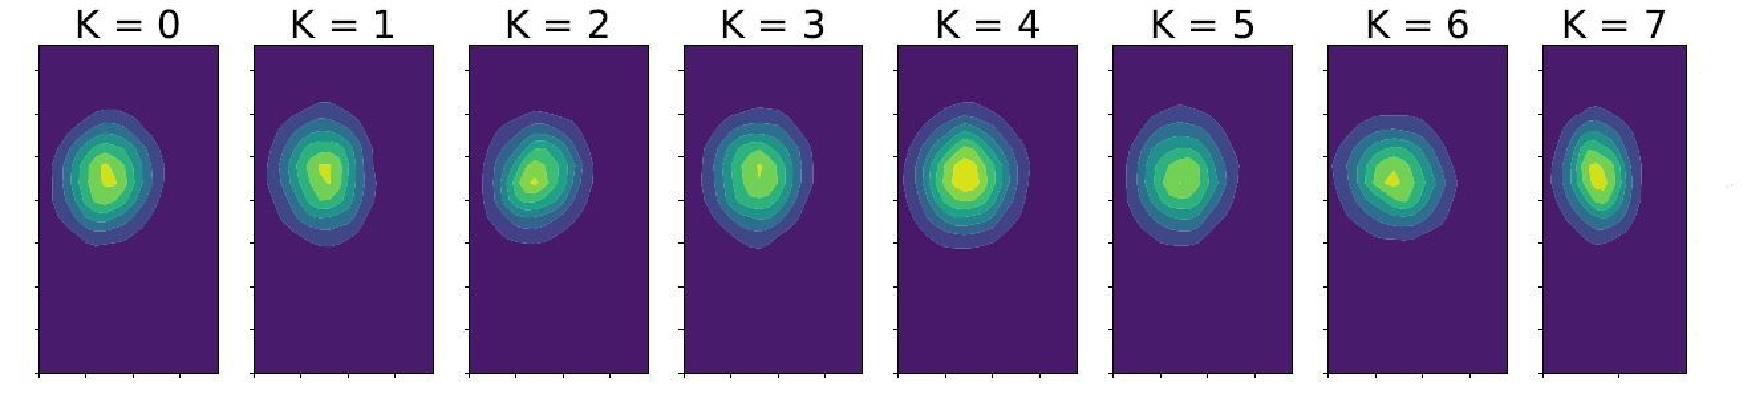
\includegraphics[width=\columnwidth]{planar_flows_plot_edited.pdf}}
		%\textbf{Inverse Autoregressive Flows}\par %\midskip
		\centerline{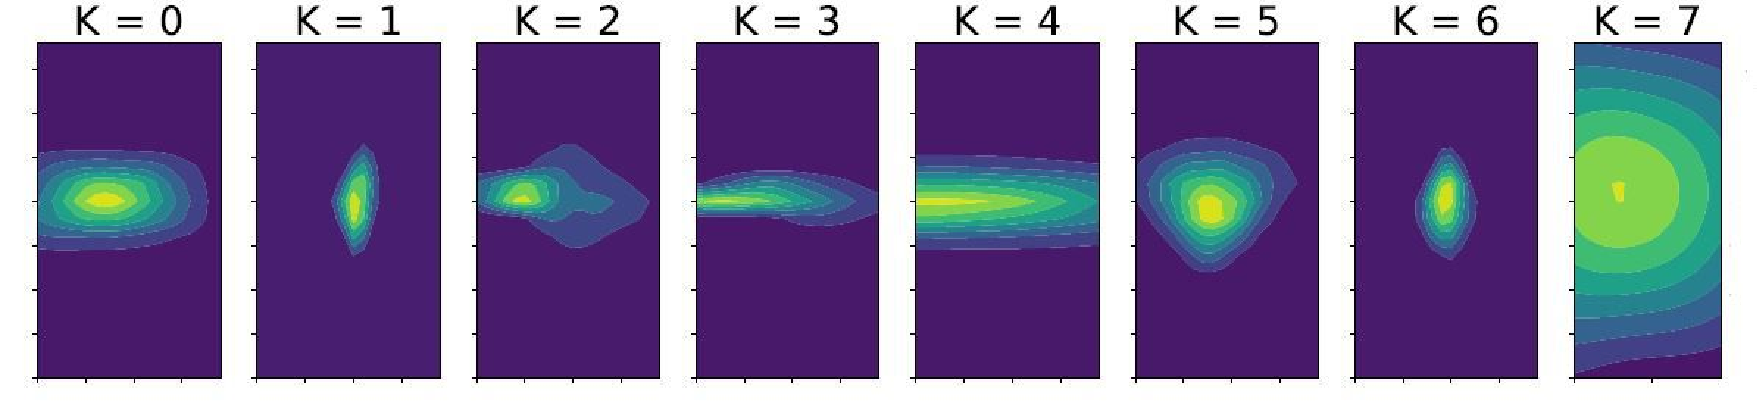
\includegraphics[width=\columnwidth]{iaf_flows_plot_edited.pdf}}
		\caption{Kernel density estimate contour plots of 10,000 samples from $q(z \cond{x, y})$ for each intermittent normalizing flow transformation of the distribution using planar (top) and \ac{IAF} (bottom) flows. The sentence pair is ``Als ich in meinen 20ern war, hatte ich meine erste Psychotherapie-Patientin." (De), translated to ``When I was in my 20s, I saw my very first psychotherapy client." (En)}
	\label{fig:flowsplot}
	\end{center}
	\vskip -0.2in
	\vspace{-4mm}
\end{figure}

We conjecture that normalizing flows are capable of helping achieve better posterior approximations of language factors, and that these improved estimates can help the expressiveness of latent codes in machine translation. Figure~\ref{fig:flowsplot} shows kernel density estimate contour plots of samples after applying normalizing flow transformation
of our distribution, as we further explain in Chapter 6 of this thesis.

%One reason for this is because of the  by introducing an additional expectation dependent on the determinant of the Jacobian of these functions, which hypothesize can allow translation systems to become more robust to a mismatch of domain.   
%As the distribution sampled from will be more complex, this 
%Another motivation for applying normalizing flows to neural machine translation is introducing additional regularization to the ELBO objective.  Some tricks to address this include KL-annealing as well as word dropout to weaken the decoder and force it to rely on the latent variable \cite{bowman2015GeneratingSent}. By incorporating normalizing flows into the objective, we hypothesize the additional regularization provided by these flows will additionally help the models from over-fitting and help prevent the latent variable from being ignored, which particularly can be useful for out-of-domain translation. 

%One other aspect much of literature has ignored is how to produce a global representation of sentences for the latent variable. The general trend has been using a mean-pooling operation over the encoder hidden states before passing the values to non-linear layer operations to produce samples from the amortized inference network \cite{Zhang2016VNMT, Su2018VRNMT, harshil2018GNMT,eikema2018AEVNMT}. We hypothesize this gives unfair weight to words-in-context that may not be as informative to capturing the meaning of sentences. As an example, consider the following two sentences: "I am happy that the dog is healthy" and "I happy dog healthy". Despite the latter being less syntatically structured, the reader would likely infer that both communicate the same underlying semantic concern for an animals well being. To investigate this in the latent variable translation setting, we apply self-attention mechanisms to the encoded states to produce weighted sums of the hidden states to determine whether this intuition is warranted or not.

Overall, we make the following contributions:
\begin{enumerate}
	\item We investigate the use of normalizing flows in \ac{LVNMT} and discuss related considerations and challenges.
	
	\item Our experiments seem to suggest that performance improvements due to the introduction of normalizing flows are minute compared to baseline models. 
	
	\item We find experimentally that when systems are trained with latent variables included, their direct contributions to final performance can be quite small. 
\end{enumerate}

%The rest of this paper is organized as follows.
%In section 2 we discuss related research. In section 3, we review previous works in latent variable machine translation and, as part of our work, we implement one such approach as a probabilistic program. For details on probabilistic programming refer to \citet{janwillem2018IntrotoProbProg}.\footnote{We do not discuss probabilistic programming in this paper, because our work is an application of such languages instead of contributions towards improving probabilistic programming.} In section 4, we discuss incorporating normalizing flows into latent variable machine translations systems and the challenges including normalizing flows. Section 5 discusses our experimental results, and we conclude in section 6. 




%    2. Main body
% Generally recommended to put each chapter into a separate file
\chapter{Background}

Hello world
\chapter{Related Work}

To our knowledge, the applications of normalizing flows have been considered sparsely in natural language processing, and largely focused on language modeling. \citet{bowman2015GeneratingSent} briefly mention normalizing flows in the context of variational auto-regressive language modeling, but did not report their empirical findings. \citet{ziegler2019LatentNFforDiscrete} provides empirical evidence on applying normalizing flows for character level language modeling. They proposed several non-autoregressive models that allow for parallel decoding, and provided evidence on the multi-modal behaviors of language factors. In this work, we focus on autoregressive approaches applied to neural machine translations.
\chapter{Methodology}


\section{Normalizing Flows for Machine Translation}

In this section we discuss incorporating normalizing flows into latent variable neural machine translation. We also discuss some challenges with incorporating normalizing flows based on the effect they have on the ELBO. 

\subsection{Applying Flows to Latent Variables}
It is relatively easy to incorporate normalizing flows into existing LVNMT models. During the training procedure, one only needs to apply $k$ functions $f_{i}$ sequentially to samples from the base distribution $p(z_{0})$: 

\begin{equation}
z_{k} = f_{k} \circ f_{k-1} ... \circ f_{2} \circ f_{1}(z_{0}) , z_{0} \sim p(z_{0})
\end{equation}

Here, $\circ$ is a shorthand for nested calls of the functions ($f_{2}(f_{1}(f_{0}(z_{0})))$). For our experiments, the base distribution $p(z_{0})$ refers to our variational distribution $q_{\phi}(\textbf{z} \cond{\textbf{x}, \textbf{y}})$ and at decode time we use $p_{\theta}(\textbf{z} \cond{\textbf{x}})$ which is the same approach taken by \citet{Zhang2016VNMT}. For deterministic decoding, we set $z_{0} = \mu_{\theta}(x)$ where $\mu_{\theta}$ is produced by our parameterized prior distribution, and apply normalizing flows on this fixed value instead of samples from $p_{\theta}(z_{0} \cond{x})$

\subsection{Challenges with Optimization}
%The one other consideration is that the inclusion of normalizing flows changes the ELBO in the following way:

%\begin{align}
%\begin{split}\label{eq:1}
%   & E_{q(z^{0}\cond{x})} [ \log p(x \cond{z^{k}}) ] - D_{KL}(q(z^{(0)} \cond{x}) || p(z^{(k)})) \\
%  &   +  E_{q(z^{0} \cond{x})} \bigg[\sum_{k=1}^{K} \log \bigg|\frac{\delta f^{(k)}}{\delta z^{(k-1)}} \bigg| \bigg]  
%\end{split}
%\end{align}

%For details on how this ELBO is derived refer to \citealp[Section 4.2]{rezende2015VIwithNF} which shows it's derivation with planar flows. Based on this formulation which was used on images, it can be written for machine translation as follows

The one other consideration with the inclusion of normalizing flows is how they change the ELBO. Here we present a formulation of the ELBO specific to machine translation which is based on the derivation from \citealp[Section 4.2]{rezende2015VIwithNF}.

\begin{align}
	\begin{split}\label{eq:2}
		&
		E_{q(\textbf{z}_{0}\cond{\textbf{x}, \textbf{y}})} \bigg[ \sum_{j=1}^{p} \log p_{\theta}(y_{j} \cond{\textbf{z}^{(k)}}, \textbf{x}, y_{<j}) \bigg] \\
		& - KL(q_{\phi}(\textbf{z}_{(0)} \cond{\textbf{x}, \textbf{y}}) || p_{\theta}(\textbf{z}^{(k)} \cond{\textbf{x}})) \\
		&   +  E_{q_{\phi}(\textbf{z}_{0} \cond{\textbf{x}, \textbf{y}})} \bigg[\sum_{k=1}^{K} \log \bigg|\frac{\delta f^{(k)}}{\delta \textbf{z}^{(k-1)}} \bigg| \bigg]  
	\end{split}
\end{align}

The first term represent maximizing the likelihood of observed sequences i.e. translating data correctly. The other two terms represent the introduced regularization from the latent variable $\textbf{z}$ in the model. 
%fyi
%https://tex.stackexchange.com/questions/44450/how-to-align-a-set-of-multiline-equations

The problem with this objective is that the inclusion of this KL divergence can lead to a problem referred to as ''posterior collapse'' \cite{he2018lagging}. This refers to the scenario where, in order to maximize the ELBO, the variational distribution parameters, for all the training data, are pushed to more closely match the prior distribution parameters. In the typical case where the prior is the unit Gaussian distribution, this leads to uninformative codes in which case the latent variable provides no additional information to the model. We recommend \citet{chen2016VariationalLossyAE} or \citet{zhao2017InfoVAE} which provide more thorough discussions on the subject. 

%The problem with this objective is that although $z_{k}$ is the product of of a number of transformations, the choice of prior $p(z)$ is still typically the unit Gaussian distribution. This choice of priors in the typical ELBO objective, has been shown to lead to the problem of ``mode collapse``, where the value of the KL term is near 0 producing uninformative latent variables. This phenomena is well documented by a number of authors, and we recommend \citet{chen2016VariationalLossyAE} or \citet{zhao2017InfoVAE} which provide more thorough discussions on the subject. 

%Although the additional expectation term for the determinant of the Jacobian encourages the model to maximize the combined shrinkage and expansion each of the flows have on the model, we still have the dependency between the original base distribution and the chosen prior distribution.  This is particularly a problem with strong generators, which refer to models flexible enough to encode all the information of the data. This could be interpreted as saying that $Y$ is independent of $Z$ at decoding time $p(Y \cond{X, Z}) = p(Y \cond{X})$.  

For this work, we address this potential problem with a previously proposed approach referred to as KL-annealing \cite{bowman2015GeneratingSent,sonderby2016LadderVAE}. KL-annealing is the process of annealing the weight associated to the divergence term in the ELBO from 0.0 (no influence) to 1.0 (original weight). We follow previous research by using a linear annealing schedule to update the weight of our regularization terms after each mini-batch update until it reaches 1.0 and the original ELBO objective is optimized for the remaining duration of training. 
%means, even if we learned a good transformation of the latent space, all our latent codes can still be uninformative and provide no additional information to the translation as all data points would essentially be samples from the prior distribution still. 

%Previous research in latent feature disentanglement has attempted to provide a theoretical understanding of this approach in the context of weaker generators through a coding theory perspective \cite{Burgess2018UnderstandingdisentBVAE}.\footnote{We note that it is unlikely that increasing the KL term above 1 would be effective in the context of disentangling features for strong generators } Other research has explored altering the Expected Lower Bound by changing the divergence term \cite{zhao2017InfoVAE}. We leave exploring alternative formulations  of the ELBO for future work as applying this objective in the context of neural machine translation (or even just recurrent neural networks)), to our knowledge, remains to be explored.

%Additionally, it should be noted that not all flows would affect the objective the same. So called "volume presevering" flows are a class of normalizing flows where the determinant of the Jacobian is equal to one. In this case, the Expectation of the absolute value of the Jacobian determinant would be a constant and we would arrive at the original ELBO objective. 

%For this work, we focus on previously proposed approaches to address this problem including KL-annealing \cite{bowman2015GeneratingSent,sonderby2016LadderVAE} and word-dropout \cite{bowman2015GeneratingSent}. KL-annealing refers to the process of increasing the weight associated to the diveregence term in the ELBO from 0.0 (no influence) to 1.0 (original weight). Typically the annealing schedule is linear, where the weight to the KL term is increased linearly after each mini-batch  until it reaches 1.0 and the original ELBO objective is optimized for the remaining duration of training. Word-drop out is an approach that involves 

%Previous research in latent feature disentanglement has attempted to provide a theoretical understanding of this approach in the context of weaker generators through a coding theory perspective \cite{Burgess2018UnderstandingdisentBVAE}.\footnote{We note that it is unlikely that increasing the KL term above 1 would be effective in the context of disentangling features for strong generators } Other research has explored altering the Expected Lower Bound by changing the divergence term \cite{zhao2017InfoVAE}. We leave exploring alternative formulations  of the ELBO for future work as applying this objective in the context of neural machine translation (or even just recurrent neural networks)), to our knowledge, remains to be explored.
\subsection{Choice of Normalizing Flows}
In the normalizing flows literature, the general trend is to find classes of invertible functions that have more computationally efficient determinants of the Jacobian. This has lead to a variety of normalizing flows available to select from which come with different trade-offs between diverse transformations and fast computation. For our experiments we consider planar flows which are discussed by \citet{rezende2015VIwithNF} and inverse autoregressive flows discussed by \citet{kingma2016IAF}. We leave exploring alternative choices of flows as future work.


%\subsection{Types of Flows}

%There are a number of different classes of normalizing flows available which seek to make calculating the determinant of the Jacobian more computationally tractable. We discuss briefly planar flows and inverse autoregressive flows which are the flows we conduct our experiments with.

%\paragraph{Planar Flows}
%Planar flows are a member of a general class of transformations of the following shape:

%\begin{equation}
%    y = z + u h(W^{T} z + b)
%\end{equation}

%where $u$, $W$, $b$ are free parameters which are learned during optimization. They can be viewed as a form of multilayer perceptron and have a nice determinant of the  Jacobian , which makes for efficient computation:

%\begin{equation}
%    |det( \frac{\partial J}{\partial z}) | = | det( 1 + u_{k}  (h'(w_{k}^{T} z_{k-1} + b_{k})w_{k} ) |
%\end{equation}

%It is difficult to determine if the time complexity gains with inverse autoregressive flows is in the context of LVNMT systems. This skepticism is in part due to previous works in latent variable translation that found a smaller dimensional latent variable vector worked better for translation.  
%In the context of latent variable machine translation, we hypothesize this flow will  adequately and the concern of a more expensive Jacobian calculation is less of a concern as smaller latent dimension vectors have shown to be sufficient in translation \cite{schulz2018StochasticDecoder}.

%NOTE: what is considered a LARGE latent space? In my mind 50 is pretty small, but is that actually the case? what if I used 10? also, forget all this KL annealing crap what if we just you know...used a smaller dimensional latent vector? the analytical form of the KL term is a sum of the dimensions so fewer dimensions means less influence on the objective. Just saying...

%\paragraph{Autoregressive Flows} 
%These are a type of normalizing flow where an autoregressive neural network conditions which transforms samples $z_{k}$ as follows:

%\begin{equation}
%    z_{k} = u_{k} + \sigma_{k} \odot z_{k-1}
%\end{equation}

%where  the the variables $u_{k}$ and $\sigma_{k}$ are the outputs of an autoregressive neural network and $\odot$ refers to the hadamard product. 

%\begin{equation}
%    u_{k,d'} , \sigma_{k, d} = \text{MLP}_{k,d} (z_{k-1, <d})
%\end{equation}

%These flows allows for linear time computation of the jacobian determinant because the Jacobian works out to be a lower triangular matrix and can be calculated in linear time as the product of the diagonal of the matrix.
\chapter{Implementation}
\chapter{Experiments}

In this chapter we discuss our experiments to evaluate performance of \ac{LVNMT} models with and without normalizing flows. We consider settings to empirically evaluate the impact of latent variables on \ac{LVNMT} systems with attention and language models. We include hyperparameter values in the supplement material Table~\ref{tab:hyperparams}, basing them mostly from \citet{eikema2018AEVNMT}. These hyperparameters were picked primarily with the generative \ac{LVNMT} system in mind, not the discriminative model. However, our main interest is not in the exact gains between models, and empirically these hyperparameters were sufficient. As part of this work, we release our code.\footnote{Experiment code:  https://github.com/gamerDecathlete/NormalizingFlowsNMT}

To help prevent \textit{posterior collapse}, we perform KL-annealing linearly over the first 80,000 mini-batch updates. We choose a word-dropout rate of 0.1 for both models. We note, previous work suggested that word dropout is not necessarily helpful in the discriminative \ac{NMT} case \cite{harshil2018GNMT}. %\reminder{depending on performance of VNMT might move to doing the pretrained trick they describe}

We conducted our experiments with the IWSLT 2016 data sets available in the \textit{torchtext} library.\footnote{https://github.com/pytorch/text} We evaluated our models with the German--English (De--En) language pair. We chose this language direction because we could more naturally evaluate the translations.\footnote{ We did not do any formal human evaluation of translation quality.} This dataset consists of 233,213 training, 2052 validation, and 9773 test sentences. We measure performance with the raw BLEU score implementation available in \textit{sacreBLEU} \cite{post2018SacreBLEU}. For all experiments, we keep the random seed fixed to a single value due to stochastic variables. %, and note that these splits are from the ones available in Torch-Text library. \reminder{move last bit to supplement material, when you do add it also note that with the current TorchText we had to manually combine data as they do not do so with the current implementation}

We represented our vocabulary for each language with \ac{BPE} \cite{sennrich2015NMTRarwordsBPE}. We used vocabularies of 10,000 \ac{BPE}s per language. We found that larger vocabularies resulted in sub-word units that occurred infrequently enough to be uninformative from a practical learning perspective. We performed \ac{BPE} using the \textit{SentencePiece} library.\footnote{https://github.com/google/sentencepiece} We trained our \ac{NMT} models on sequences of maximum length 50. We used beam search with a beam width of 10, and length normalization set to 1.0. Throughout our experiments we will refer to our discriminative models as \ac{VNMT} and our joint system as \ac{GNMT}. % The only other normalizing we did on our data sets was removing diacritics from the Arabic sentences. 


%Although most research in \ac{NMT} literature use beam search decoding, we choose to to use greedy decoding when translating sentences. Our general assumption is that if normalizing flows help with translation, this would carry over to heuristic searchers like beam search. Also, in recent literature studying the impact of beam search, larger beams do not necessarily translate to providing huge improvements in performance \cite{cohen2019unconstrained}. \reminder{ this...is a cop out midly because I saw performance degredation with my beam search algorithm set to 10... it worked fine on a 4,000,000 mil sentence dataset but that took waaaay to long}

%- Our networks use hidden layer sizes and embeddings of size 256 which is similar to the choices made in [eikeman et. al 2018] and we found for VNMT these parameters also worked better than those in [vnmt et. al.] for preliminary experiments on the WMT 2014 data they evaluated on. All specific params are in supplement material.
%We limit ourselves to these datasets, because it allows us to consider multiple language pairs and is a manageable size for our available computation budget. Due to these constraints, we caution readers that our results may not be applicable to datasets of different sizes.

\section{General Translation}

In this section we report our results when including normalizing flows on top of \ac{LVNMT} systems. Our hypothesis was that, given normalizing flows success in computer vision, similar gains can be achieved by including normalizing flows in previously considered \ac{LVNMT} systems.  

%\reminder{ in table 1 dimension of Z = 2, with planar flows set to 2 we get so and so results. (point to cells in table)}
%\reminder{ with latent dim = 2, flows do not really offer any improvement, but if you go with a higher dim space, results suggest adding flows can improve performance. Smaller latent space, GNMT is better without flows, but VNMT benefits from normalizing flows. If we go to higher dimension we start to see some gains with GNMT. Pattern: Planar flows usually do well with a higher number of flows seem to help where as IAF helps with smaller flow }

Our baselines include the \ac{LVNMT} models we described in Chapter 3 with just the diagonal Gaussian for the variational distribution. Our baselines optimize the \ac{ELBO} with an equal number of \ac{MC} samples as our normalizing flows models to provide a fair comparison. This corresponds to better approximations of the negative log-likelihood of sequence predictions. The KL divergence is analytic in the Gaussian case which does not require sampling \cite{kingma2014autoencodingVB,rezende2014stochasticBackprop}. Although we do not report numbers, we did find just increasing the number of \ac{MC} samples improved translation quality on the validation set.

Table \ref{tab:de_en_besttranslations} shows the BLEU score of our results on the test set. The best model was picked based on validation BLEU score from checkpoints after every epoch of training. Each model was trained for 47 epochs.\footnote{An epoch here refers to training on all mini-batches before reshuffling the sentence pairs.} The boldfaced results represent the best performing version of a model for the given latent dimensions and flow type.

Regardless of flow type, we found our generative model to perform better for any number of flows or latent space size. Even our worst performing \ac{GNMT} model (z=128, with 4 Planar flows) provides at least 1.20 BLEU score above the best performing discriminative model (z=128, with 4 \ac{IAF}). This result seems congruent with previous research suggesting joint modelling can be more effective than the simpler discriminative representation \cite{eikema2018AEVNMT}.

We found overall that \ac{VNMT} benefited more from the inclusion of normalizing flows than \ac{GNMT}. For \ac{VNMT}, even a single normalizing flow results in improvements. Between flows, we do not note any clear distinctions for the number of flows or type of flow in the \ac{VNMT} case although best performance included more than just one flow. In contrast, \ac{GNMT} only saw performance gains with a latent space of 256, and even then only a few of the flows models outperformed the baseline. 

Overall these results suggest that flows can indeed be added to existing models and provide benefit to the final translation quality. In several instances our flows models outperform baseline results. Here, it seems the input feeding \ac{VNMT} may benefit more than the initialization approach in our \ac{GNMT} model.

%Our results seem to confirm previous findings on transform complexity, when comparing the flow type for a given number of flows for latent spaces 128 and 256. Generally the \ac{IAF} flows gave higher BLEU score with fewer flows compared to the same number of planar flows. This seems to affirm previous research showing that more complex flows require fewer layers to be beneficial \cite{kingma2016IAF,Berg2018SylvesterNF}. However, as we begin using higher numbers of flows we find that planar flows begin to perform marginally better. This would seem to highlight research suggesting better amortization schemes of flow parameters can generally be beneficial \cite{Berg2018SylvesterNF}, as well the limitations of planar flows transformation capabilities \cite{rezende2015VIwithNF,Berg2018SylvesterNF}.




\begin{table}[] 
	\caption{BLEU score for our models with normalizing flows for German-English (De--En) translation. The best  performances are in bold as compared to differing numbers of flows and the baseline. Yellow rows represent our \ac{VNMT} model results, and red our \ac{GNMT} results for differing number and type of flows. 
		% \reminder{0 flows IS my baseline, explain what your basleines are in. Bold baseline 1 (column explainin it), baseline 2 (column explainin what it is?) }
		 }
	\center
	\label{tab:de_en_besttranslations}
	\begin{tabular}{llllllcl}
		\multicolumn{8}{c}{\textbf{Latent Dimension: 128}}                                                                                                                                                                                                                                                                                                                                                                                                                                                                                                 \\ \hline
		\multicolumn{1}{|l|}{\textbf{Flows}}                          & \multicolumn{1}{l|}{\textbf{1}}                             & \multicolumn{1}{l|}{\textbf{2}}                             & \multicolumn{1}{l|}{\textbf{4}}                             & \multicolumn{1}{l|}{\textbf{8}}                             & \multicolumn{1}{l|}{\textbf{16}}                            & \multicolumn{1}{l|}{\textbf{0 (Baseline)}}                                    & \multicolumn{1}{l|}{\textbf{Model}}                                          \\ \hline
		\rowcolor[HTML]{F9F9E1} 
		\multicolumn{1}{|l|}{\cellcolor[HTML]{F9F9E1}Planar}          & \multicolumn{1}{l|}{\cellcolor[HTML]{F9F9E1}18.84}          & \multicolumn{1}{l|}{\cellcolor[HTML]{F9F9E1}18.84}          & \multicolumn{1}{l|}{\cellcolor[HTML]{F9F9E1}19.14}          & \multicolumn{1}{l|}{\cellcolor[HTML]{F9F9E1}19.02}          & \multicolumn{1}{l|}{\cellcolor[HTML]{F9F9E1}\textbf{19.18}} & \multicolumn{1}{c|}{\cellcolor[HTML]{F9F9E1}}                                 & \multicolumn{1}{l|}{\cellcolor[HTML]{F9F9E1}}                                \\ \cline{1-6}
		\rowcolor[HTML]{F9F9E1} 
		\multicolumn{1}{|l|}{\cellcolor[HTML]{F9F9E1}IAF}             & \multicolumn{1}{l|}{\cellcolor[HTML]{F9F9E1}18.89}          & \multicolumn{1}{l|}{\cellcolor[HTML]{F9F9E1}18.96}          & \multicolumn{1}{l|}{\cellcolor[HTML]{F9F9E1}\textbf{19.29}} & \multicolumn{1}{l|}{\cellcolor[HTML]{F9F9E1}18.81}          & \multicolumn{1}{l|}{\cellcolor[HTML]{F9F9E1}18.92}          & \multicolumn{1}{c|}{\multirow{-2}{*}{\cellcolor[HTML]{F9F9E1}18.768}}         & \multicolumn{1}{l|}{\multirow{-2}{*}{\cellcolor[HTML]{F9F9E1}VNMT}}          \\ \hline
		\rowcolor[HTML]{F4DAD8} 
		\multicolumn{1}{|l|}{\cellcolor[HTML]{F4DAD8}Planar}          & \multicolumn{1}{l|}{\cellcolor[HTML]{F4DAD8}20.59}          & \multicolumn{1}{l|}{\cellcolor[HTML]{F4DAD8}20.60}          & \multicolumn{1}{l|}{\cellcolor[HTML]{F4DAD8}20.48}          & \multicolumn{1}{l|}{\cellcolor[HTML]{F4DAD8}20.55}          & \multicolumn{1}{l|}{\cellcolor[HTML]{F4DAD8}20.66}          & \multicolumn{1}{c|}{\cellcolor[HTML]{F4DAD8}}                                 & \multicolumn{1}{l|}{\cellcolor[HTML]{F4DAD8}}                                \\ \cline{1-6}
		\rowcolor[HTML]{F4DAD8} 
		\multicolumn{1}{|l|}{\cellcolor[HTML]{F4DAD8}IAF}             & \multicolumn{1}{l|}{\cellcolor[HTML]{F4DAD8}20.64}          & \multicolumn{1}{l|}{\cellcolor[HTML]{F4DAD8}20.64}          & \multicolumn{1}{l|}{\cellcolor[HTML]{F4DAD8}20.51}          & \multicolumn{1}{l|}{\cellcolor[HTML]{F4DAD8}20.65}          & \multicolumn{1}{l|}{\cellcolor[HTML]{F4DAD8}20.50}          & \multicolumn{1}{c|}{\multirow{-2}{*}{\cellcolor[HTML]{F4DAD8}\textbf{20.73}}} & \multicolumn{1}{l|}{\multirow{-2}{*}{\cellcolor[HTML]{F4DAD8}GNMT}}          \\ \hline
		\multicolumn{8}{c}{\textbf{Latent Dimension: 256}}                                                                                                                                                                                                                                                                                                                                                                                                                                                                                                 \\ \hline
		\multicolumn{1}{|l|}{\textbf{Flows}}                          & \multicolumn{1}{l|}{\textbf{1}}                             & \multicolumn{1}{l|}{\textbf{2}}                             & \multicolumn{1}{l|}{\textbf{4}}                             & \multicolumn{1}{l|}{\textbf{8}}                             & \multicolumn{1}{l|}{\textbf{16}}                            & \multicolumn{1}{l|}{\textbf{0 (Baseline)}}                                    & \multicolumn{1}{l|}{\textbf{Model}}                                          \\ \hline
		\rowcolor[HTML]{F9F9E1} 
		\multicolumn{1}{|l|}{\cellcolor[HTML]{F9F9E1}Planar} & \multicolumn{1}{l|}{\cellcolor[HTML]{F9F9E1}18.93}          & \multicolumn{1}{l|}{\cellcolor[HTML]{F9F9E1}\textbf{19.26}} & \multicolumn{1}{l|}{\cellcolor[HTML]{F9F9E1}19.02}          & \multicolumn{1}{l|}{\cellcolor[HTML]{F9F9E1}18.80}          & \multicolumn{1}{l|}{\cellcolor[HTML]{F9F9E1}18.82}          & \multicolumn{1}{c|}{\cellcolor[HTML]{F9F9E1}}                                 & \multicolumn{1}{l|}{\cellcolor[HTML]{F9F9E1}}                                \\ \cline{1-6}
		\rowcolor[HTML]{F9F9E1} 
		\multicolumn{1}{|l|}{\cellcolor[HTML]{F9F9E1}IAF}    & \multicolumn{1}{l|}{\cellcolor[HTML]{F9F9E1}18.95}          & \multicolumn{1}{l|}{\cellcolor[HTML]{F9F9E1}\textbf{19.17}} & \multicolumn{1}{l|}{\cellcolor[HTML]{F9F9E1}19.02}          & \multicolumn{1}{l|}{\cellcolor[HTML]{F9F9E1}18.99}          & \multicolumn{1}{l|}{\cellcolor[HTML]{F9F9E1}18.77}          & \multicolumn{1}{c|}{\multirow{-2}{*}{\cellcolor[HTML]{F9F9E1}18.76}}          & \multicolumn{1}{l|}{\multirow{-2}{*}{\cellcolor[HTML]{F9F9E1}VNMT}} \\ \hline
		\rowcolor[HTML]{F4DAD8} 
		\multicolumn{1}{|l|}{\cellcolor[HTML]{F4DAD8}Planar} & \multicolumn{1}{l|}{\cellcolor[HTML]{F4DAD8}20.55}          & \multicolumn{1}{l|}{\cellcolor[HTML]{F4DAD8}\textbf{20.67}} & \multicolumn{1}{l|}{\cellcolor[HTML]{F4DAD8}20.54}          & \multicolumn{1}{l|}{\cellcolor[HTML]{F4DAD8}20.51}          & \multicolumn{1}{l|}{\cellcolor[HTML]{F4DAD8}\textbf{20.67}} & \multicolumn{1}{c|}{\cellcolor[HTML]{F4DAD8}}                                 & \multicolumn{1}{l|}{\cellcolor[HTML]{F4DAD8}}                                \\ \cline{1-6}
		\rowcolor[HTML]{F4DAD8} 
		\multicolumn{1}{|l|}{\cellcolor[HTML]{F4DAD8}IAF}    & \multicolumn{1}{l|}{\cellcolor[HTML]{F4DAD8}20.85}          & \multicolumn{1}{l|}{\cellcolor[HTML]{F4DAD8}\textbf{20.86}} & \multicolumn{1}{l|}{\cellcolor[HTML]{F4DAD8}20.64}          & \multicolumn{1}{l|}{\cellcolor[HTML]{F4DAD8}20.62}          & \multicolumn{1}{l|}{\cellcolor[HTML]{F4DAD8}20.66}          & \multicolumn{1}{c|}{\multirow{-2}{*}{\cellcolor[HTML]{F4DAD8}20.66}}          & \multicolumn{1}{l|}{\multirow{-2}{*}{\cellcolor[HTML]{F4DAD8}GNMT}} \\ \hline
	\end{tabular}
\end{table}

%For our baselines, we train both a VNMT and VAENMT model without normalizing flows. To provide equal comparisons we use the same number of samples as our normalizing flows models. In [Eqn for elbo] this corresponds to better approximations to the negative log-likelihood of sequence predictions as the KL divergence is analytic in the Gaussian case \cite{kingma, }. We consider latent dimensions of 2, 128 [best working latent space in Schulz et. al. 2018 for VNMT], and 256 [value used in Eikman et. al. model]. We consider latent dimensions of 2 as we plot the latent space with normalizing flows, and have previously seen this number of latent dimensions to perform quite well compared to large latent dimensions. We use a linear annealing schedule over the first 2 epochs of training to encourage both models to rely on the latent variables which has been shown to improve overall performance [cite cite cite]. We also try without any annealing to provide a comparison on gains from this annealing. We abstain from using word-dropout which is another regularization technique others have found useful previously to help with some models. Particularly in the VNMT case [GNMT paper] found that it did not help improve performance that particular system. 

%To evaluate our hypothesis, we then include normalizing flows on top of these existing systems keeping everything else in the system fixed. We again consider no annealing and annealing for 2 epochs, and train with N number of samples to approximate the ELBO during the training process. We consider 1, 2, 4, 8, and 16 flows to see if performance improves with an increasing number of flows. We test on the inverse autoregressive flows, and amortized planar flows available in the Pyro library. [might also consider Sylvester flows depending on the results from these...would require a smidge of implementing the amortization].

%We evaluate performance on the BLEU score and also measure the (-ELBO) and NLL during training to determine performance gains from normalizing flows. 




\section{Importance of Attention}

In this section, to investigate the utility of including latent variables, we train simplified versions of our \ac{LVNMT} systems which do not include the attention mechanism. Our motivation for this experiment is to tease apart the impact of our latent variable as the only additional information to the decoding process. We do not expect this system to outperform the models with attention due to their success in \ac{SOTA} models \cite{bahdanau2014NMTBYJoint, vaswani2017attentionTransformer}. However, we hypothesize that if the latent variable can encode useful information in translation, then \ac{NMT} models will still benefit from this global latent information. As an extension, normalizing flows will then enable these variables to be more beneficial by making the latent variable distribution more flexible.

We include the latent variable in the generator network as a substitute for attention, which is the same design choice as \citet{bahdanau2014NMTBYJoint} for including attention. In our previous experiment we did not consider this, as the focus was on incorporating normalizing flows in variations of existing models. We compare our modified discriminative model against a version of \citet{bahdanau2014NMTBYJoint} where attention is simply removed. In the joint modelling case, we compare to a baseline similar to the joint model of \citet{eikema2018AEVNMT} except without attention. Their model optimize the language model and translation systems separately except for sharing the source language word embeddings. All other hyperparameters are the same. In our tables these two modified models are the No Latent (NL) baselines we compare our latent variable models against. Table \ref{tab:de_en_no_attention} show's results for our modified models and the baselines when evaluated with BLEU score. The best performances are bold. They were chosen by comparing models with differing numbers of the same flow, and the baselines.

Considering only the latent dimension size, we find an increase in performance simply doubling the dimensions of the latent variable. This would suggest that bigger latent spaces become more important when the model depends more on the latent variable. The combination of planar flows and \ac{VNMT} seem to benefit most from the latent variable achieving close to our best \ac{GNMT} baseline. Unfortunately, the \ac{IAF} \ac{VNMT} models did not improve as much. There could be several possible reasons. One interpretation we suspect is related to the data conditioning approach of planar flows compared to \ac{IAF}. As our planar flows provide per-sentence flow parameters, this enables them to provide more unique distributions per sentence. In comparison, the \ac{IAF} is unable to capture this more nuanced information by simply conditioning on a context vector. This argument has been pointed out in previous research for other types of flow \cite{Berg2018SylvesterNF}.

Unfortunately, our \ac{GNMT} model did not benefit from the inclusion of normalizing flows and was actually hindered in performance for most choices of flows. We reason this is due to the formulation of \ac{GNMT}. The latent variable initializes the translation system beginning in the encoder network as compared to being passed as input during decoding. Based on our results, it seems this design is less effective compared to the input feeding approach of \ac{VNMT} to utilize latent variables. We conjecture this is likely without explicitly passing $z$ to the decoder, \ac{GNMT} is relying on the \ac{GRU}s to implicitly keep this information from beginning to end. 


\begin{table}[]
	\caption{Results for translation systems without attention mechanism. Baseline includes models with normalizing flows and deterministic version of model excluding latent variables. \ac{VNMT} results are in yellow, and \ac{GNMT} results are in red with best models.  Best models across number and type of flow are in bold. No Latent (NL) are  models trained without z included.
		}
	\label{tab:de_en_no_attention}
	\center
	\begin{tabular}{llllllccl}
		\multicolumn{9}{c}{\textbf{Latent Dimension: 128}}                                                                                                                                                                                                                                                                                                                                                                                                                                                                                                                             \\ \hline
		\multicolumn{1}{|c|}{\textbf{Flows}}                 & \multicolumn{1}{c|}{\textbf{1}}                            & \multicolumn{1}{c|}{\textbf{2}}                   & \multicolumn{1}{c|}{\textbf{4}}                   & \multicolumn{1}{c|}{\textbf{8}}                   & \multicolumn{1}{c|}{\textbf{16}}                           & \multicolumn{1}{c|}{\textbf{0 (Baseline)}}                                   & \multicolumn{1}{c|}{\textbf{NL (Baseline)}}                  & \multicolumn{1}{c|}{\textbf{Model}}                                          \\ \hline
		\rowcolor[HTML]{F9F9E1} 
		\multicolumn{1}{|l|}{\cellcolor[HTML]{F9F9E1}Planar} & \multicolumn{1}{l|}{\cellcolor[HTML]{F9F9E1}6.61}          & \multicolumn{1}{l|}{\cellcolor[HTML]{F9F9E1}6.64} & \multicolumn{1}{l|}{\cellcolor[HTML]{F9F9E1}6.63} & \multicolumn{1}{l|}{\cellcolor[HTML]{F9F9E1}6.93} & \multicolumn{1}{l|}{\cellcolor[HTML]{F9F9E1}\textbf{6.78}} & \multicolumn{1}{c|}{\cellcolor[HTML]{F9F9E1}}                                & \multicolumn{1}{c|}{\cellcolor[HTML]{F9F9E1}}                       & \multicolumn{1}{l|}{\cellcolor[HTML]{F9F9E1}}                                \\ \cline{1-6}
		\rowcolor[HTML]{F9F9E1} 
		\multicolumn{1}{|l|}{\cellcolor[HTML]{F9F9E1}IAF}    & \multicolumn{1}{l|}{\cellcolor[HTML]{F9F9E1}\textbf{6.42}} & \multicolumn{1}{l|}{\cellcolor[HTML]{F9F9E1}6.32} & \multicolumn{1}{l|}{\cellcolor[HTML]{F9F9E1}6.28} & \multicolumn{1}{l|}{\cellcolor[HTML]{F9F9E1}5.98} & \multicolumn{1}{l|}{\cellcolor[HTML]{F9F9E1}5.92}          & \multicolumn{1}{c|}{\multirow{-2}{*}{\cellcolor[HTML]{F9F9E1}6.25}}          & \multicolumn{1}{c|}{\multirow{-2}{*}{\cellcolor[HTML]{F9F9E1}6.38}} & \multicolumn{1}{l|}{\multirow{-2}{*}{\cellcolor[HTML]{F9F9E1}VNMT}}          \\ \hline
		\rowcolor[HTML]{F4DAD8} 
		\multicolumn{1}{|l|}{\cellcolor[HTML]{F4DAD8}Planar} & \multicolumn{1}{l|}{\cellcolor[HTML]{F4DAD8}7.2}           & \multicolumn{1}{l|}{\cellcolor[HTML]{F4DAD8}7.22} & \multicolumn{1}{l|}{\cellcolor[HTML]{F4DAD8}7.19} & \multicolumn{1}{l|}{\cellcolor[HTML]{F4DAD8}7.11} & \multicolumn{1}{l|}{\cellcolor[HTML]{F4DAD8}7.25}          & \multicolumn{1}{c|}{\cellcolor[HTML]{F4DAD8}\textbf{7.37}}                   & \multicolumn{1}{c|}{\cellcolor[HTML]{F4DAD8}}                       & \multicolumn{1}{l|}{\cellcolor[HTML]{F4DAD8}}                                \\ \cline{1-7}
		\rowcolor[HTML]{F4DAD8} 
		\multicolumn{1}{|l|}{\cellcolor[HTML]{F4DAD8}IAF}    & \multicolumn{1}{l|}{\cellcolor[HTML]{F4DAD8}7.31}          & \multicolumn{1}{l|}{\cellcolor[HTML]{F4DAD8}7.37} & \multicolumn{1}{l|}{\cellcolor[HTML]{F4DAD8}7.33} & \multicolumn{1}{l|}{\cellcolor[HTML]{F4DAD8}7.18} & \multicolumn{1}{l|}{\cellcolor[HTML]{F4DAD8}\textbf{7.41}} & \multicolumn{1}{c|}{\cellcolor[HTML]{F4DAD8}7.37}                            & \multicolumn{1}{c|}{\multirow{-2}{*}{\cellcolor[HTML]{F4DAD8}7.16}} & \multicolumn{1}{l|}{\multirow{-2}{*}{\cellcolor[HTML]{F4DAD8}GNMT}}          \\ \hline
		\multicolumn{9}{c}{\textbf{Latent Dimension: 256}}                                                                                                                                                                                                                                                                                                                                                                                                                                                                                                                             \\ \hline
		\multicolumn{1}{|c|}{\textbf{Flows}}                 & \multicolumn{1}{c|}{\textbf{1}}                            & \multicolumn{1}{c|}{\textbf{2}}                   & \multicolumn{1}{c|}{\textbf{4}}                   & \multicolumn{1}{c|}{\textbf{8}}                   & \multicolumn{1}{c|}{\textbf{16}}                           & \multicolumn{1}{c|}{\textbf{0 (Baseline)}}                                   & \multicolumn{1}{c|}{\textbf{NL (Baseline)}}                  & \multicolumn{1}{c|}{\textbf{Model}}                                          \\ \hline
		\rowcolor[HTML]{F9F9E1} 
		\multicolumn{1}{|l|}{\cellcolor[HTML]{F9F9E1}Planar} & \multicolumn{1}{l|}{\cellcolor[HTML]{F9F9E1}6.31}          & \multicolumn{1}{l|}{\cellcolor[HTML]{F9F9E1}6.81} & \multicolumn{1}{l|}{\cellcolor[HTML]{F9F9E1}6.91} & \multicolumn{1}{l|}{\cellcolor[HTML]{F9F9E1}7.37} & \multicolumn{1}{l|}{\cellcolor[HTML]{F9F9E1}\textbf{7.38}} & \multicolumn{1}{c|}{\cellcolor[HTML]{F9F9E1}}                                & \multicolumn{1}{c|}{\cellcolor[HTML]{F9F9E1}}                       & \multicolumn{1}{l|}{\cellcolor[HTML]{F9F9E1}}                                \\ \cline{1-6}
		\rowcolor[HTML]{F9F9E1} 
		\multicolumn{1}{|l|}{\cellcolor[HTML]{F9F9E1}IAF}    & \multicolumn{1}{l|}{\cellcolor[HTML]{F9F9E1}6.45}          & \multicolumn{1}{l|}{\cellcolor[HTML]{F9F9E1}6.47} & \multicolumn{1}{l|}{\cellcolor[HTML]{F9F9E1}6.4}  & \multicolumn{1}{l|}{\cellcolor[HTML]{F9F9E1}6.23} & \multicolumn{1}{l|}{\cellcolor[HTML]{F9F9E1}\textbf{6.71}} & \multicolumn{1}{c|}{\multirow{-2}{*}{\cellcolor[HTML]{F9F9E1}6.43}}          & \multicolumn{1}{c|}{\multirow{-2}{*}{\cellcolor[HTML]{F9F9E1}6.38}} & \multicolumn{1}{l|}{\multirow{-2}{*}{\cellcolor[HTML]{F9F9E1}VNMT}} \\ \hline
		\rowcolor[HTML]{F4DAD8} 
		\multicolumn{1}{|l|}{\cellcolor[HTML]{F4DAD8}Planar} & \multicolumn{1}{l|}{\cellcolor[HTML]{F4DAD8}7.4}           & \multicolumn{1}{l|}{\cellcolor[HTML]{F4DAD8}7.22} & \multicolumn{1}{l|}{\cellcolor[HTML]{F4DAD8}7.33} & \multicolumn{1}{l|}{\cellcolor[HTML]{F4DAD8}7.26} & \multicolumn{1}{l|}{\cellcolor[HTML]{F4DAD8}7.07}          & \multicolumn{1}{c|}{\cellcolor[HTML]{F4DAD8}}                                & \multicolumn{1}{c|}{\cellcolor[HTML]{F4DAD8}}                       & \multicolumn{1}{l|}{\cellcolor[HTML]{F4DAD8}}                                \\ \cline{1-6}
		\rowcolor[HTML]{F4DAD8} 
		\multicolumn{1}{|l|}{\cellcolor[HTML]{F4DAD8}IAF}    & \multicolumn{1}{l|}{\cellcolor[HTML]{F4DAD8}7.35}          & \multicolumn{1}{l|}{\cellcolor[HTML]{F4DAD8}7.34} & \multicolumn{1}{l|}{\cellcolor[HTML]{F4DAD8}7.28} & \multicolumn{1}{l|}{\cellcolor[HTML]{F4DAD8}7.04} & \multicolumn{1}{l|}{\cellcolor[HTML]{F4DAD8}7.36}          & \multicolumn{1}{c|}{\multirow{-2}{*}{\cellcolor[HTML]{F4DAD8}\textbf{7.51}}} & \multicolumn{1}{c|}{\multirow{-2}{*}{\cellcolor[HTML]{F4DAD8}7.16}} & \multicolumn{1}{l|}{\multirow{-2}{*}{\cellcolor[HTML]{F4DAD8}GNMT}} \\ \hline
	\end{tabular}
\end{table}

\section{Understanding Latent Variable} 

%Hypothesis: If the latent variable is encoding information important to the translation process, it stands to reason setting Z = [0, 0 ,.... 0] during the evaluation process will negatively impact translation performance, as otherwise the latent variable z is not encoding useful information in the system.

%Previous research which incorporate latent variables in \ac{NMT} systems have often focused on non-zero KL values as justification for the latent variable encoding information for the generative system. The argument in favor of this metric is that the magnitude of the KL can be used a heuristic to gauge the importance the latent variable plays in the translation system. This stems from the fact that typically the prior is a stationary target and if the KL term is small that the latent variable is uninformative to the system's performance. A limitation of this measurement is that it is not applicable in situation where the prior is learned jointly, such as in our \ac{VNMT} system.

In previous works, the utility of latent variables is typically justified by training a similar system without the latent variable included, or by optimizing the model differently.  In cases where the prior is stationary, authors then typically report the KL divergence to justify the latent variables usage. This metric is inapplicable to \ac{VNMT} where the prior is learned. In the ideal \ac{VNMT} scenario, the KL divergence being 0 suggests both distributions encode the same information.

As an alternative approach to measure the value of our latent variable during translation, we set $z$ to the 0 vector. We measure the difference in BLEU score with and without $z$ during the decoding process. This can give us direct insight into the importance of $z$ when translating sentences, whether the prior is learned or not. Table~\ref{tab:de_en_kl_divergence} provides the KL divergence and Table~\ref{tab:de_en_delta_bleu} shows the difference in BLEU score when z is the 0 vector for our models with attention. 

Interestingly, for many of our \ac{VNMT} models with planar flows we see including $z$ often negatively impacts performance of the translation system. This could suggest that the latent variable itself is not helping the translation, but improves representations in the encoder or source word embeddings. Another explanation is that our substitution of $p_{\theta}$ for $q_{\phi}$ at decode time provide information that is too dissimilar to the variational distribution. This is plausible given that in many cases the KL divergence is non-zero, but even in several instances a lower KL divergence still leads to loss of performance with z (see \ac{VNMT}, z=256 results for 8 flows vs. 16 flows). These substitution approaches have also previously been shown to provide minimal or mixed results in terms of comparative performance \cite{eikema2018AEVNMT}.

The exception to our above observations of course is our \ac{VNMT} with \ac{IAF} models in higher dimensions which seem to heavily depend on the latent variable. One possible reason for this has to do with the amortization of \ac{IAF} flows. As these flows are composed of neural networks shared across data points, they can more easily be viewed as additional layers in the network.\footnote{In a similar setting, one bug we found in our implementation was excluding the projection layer and found similar performance drops to those without \ac{IAF} flows results.} This could also be a more volatile result which occurs due to different choices of initialization. It has been noted KL annealing schemes can be affected by initialization for final performance \cite{sphericallatent2018Xu}.

In comparison, \ac{GNMT} seems to generally show at least minute dependence on the latent variable regardless of number of flows. There do not seem to be any clear patterns between choices about flows and the information encoded by $z$. Likewise, a higher KL divergence does not necessarily correspond to more utility in translation performance.  

When we perform the same experiment with our \ac{LVNMT} systems without attention, we see more dependence on the latent variable for all models. Our results are in Table~\ref{tab:de_en_no_attention_kl_div} and \ref{tab:de_en_no_attention_delta_bleu}. In most cases with planar flows, we see our models depend more on the latent variable over the baseline without planar flows. Our \ac{IAF} flow models are more mixed in terms of performance changes, where in \ac{GNMT} our models depend more on the flows with a smaller latent dimension space as opposed to larger latent space. 

\begin{table}
	\caption{Average KL divergence for the test set. For \ac{VNMT} (yellow) the KL term should be smaller, meaning the distributions encode similar information. For \ac{GNMT} (red) they should be higher as these suggest more informative latent spaces.  }
	\label{tab:de_en_kl_divergence}
	\center
	\begin{tabular}{lccccccl}
		\multicolumn{8}{c}{\textbf{Latent Dimension: 128 (KL Divergence)}}                                                                                                \\ \hline
		\multicolumn{1}{|l|}{\textbf{Flows}}                       & \multicolumn{1}{c|}{\textbf{1}}                   & \multicolumn{1}{c|}{\textbf{2}}                   & \multicolumn{1}{c|}{\textbf{4}}                    & \multicolumn{1}{c|}{\textbf{8}}                   & \multicolumn{1}{c|}{\textbf{16}}                   & \multicolumn{1}{c|}{\textbf{0 (Baseline)}}                          & \multicolumn{1}{l|}{\textbf{Model}}                                          \\ \hline
		\rowcolor[HTML]{F9F9E1} 
		\multicolumn{1}{|l|}{\cellcolor[HTML]{F9F9E1}Planar}       & \multicolumn{1}{c|}{\cellcolor[HTML]{F9F9E1}2.16} & \multicolumn{1}{c|}{\cellcolor[HTML]{F9F9E1}1.27} & \multicolumn{1}{c|}{\cellcolor[HTML]{F9F9E1}1.18}  & \multicolumn{1}{c|}{\cellcolor[HTML]{F9F9E1}1.04} & \multicolumn{1}{c|}{\cellcolor[HTML]{F9F9E1}1.63}  & \multicolumn{1}{c|}{\cellcolor[HTML]{F9F9E1}}                       & \multicolumn{1}{l|}{\cellcolor[HTML]{F9F9E1}}                                \\ \cline{1-6}
		\rowcolor[HTML]{F9F9E1} 
		\multicolumn{1}{|l|}{\cellcolor[HTML]{F9F9E1}IAF}          & \multicolumn{1}{c|}{\cellcolor[HTML]{F9F9E1}0.68} & \multicolumn{1}{c|}{\cellcolor[HTML]{F9F9E1}1.35} & \multicolumn{1}{c|}{\cellcolor[HTML]{F9F9E1}1.32}  & \multicolumn{1}{c|}{\cellcolor[HTML]{F9F9E1}1.6}  & \multicolumn{1}{c|}{\cellcolor[HTML]{F9F9E1}1.06}  & \multicolumn{1}{c|}{\multirow{-2}{*}{\cellcolor[HTML]{F9F9E1}1.04}} & \multicolumn{1}{l|}{\multirow{-2}{*}{\cellcolor[HTML]{F9F9E1}VNMT}}          \\ \hline
		\rowcolor[HTML]{F4DAD8} 
		\multicolumn{1}{|l|}{\cellcolor[HTML]{F4DAD8}Planar}       & \multicolumn{1}{c|}{\cellcolor[HTML]{F4DAD8}3.23} & \multicolumn{1}{c|}{\cellcolor[HTML]{F4DAD8}3.15} & \multicolumn{1}{c|}{\cellcolor[HTML]{F4DAD8}2.36}  & \multicolumn{1}{c|}{\cellcolor[HTML]{F4DAD8}2.82} & \multicolumn{1}{c|}{\cellcolor[HTML]{F4DAD8}3.64}  & \multicolumn{1}{c|}{\cellcolor[HTML]{F4DAD8}}                       & \multicolumn{1}{l|}{\cellcolor[HTML]{F4DAD8}}                                \\ \cline{1-6}
		\rowcolor[HTML]{F4DAD8} 
		\multicolumn{1}{|l|}{\cellcolor[HTML]{F4DAD8}IAF}          & \multicolumn{1}{c|}{\cellcolor[HTML]{F4DAD8}4.31} & \multicolumn{1}{c|}{\cellcolor[HTML]{F4DAD8}4.36} & \multicolumn{1}{c|}{\cellcolor[HTML]{F4DAD8}4.19}  & \multicolumn{1}{c|}{\cellcolor[HTML]{F4DAD8}4.43} & \multicolumn{1}{c|}{\cellcolor[HTML]{F4DAD8}4.14}  & \multicolumn{1}{c|}{\multirow{-2}{*}{\cellcolor[HTML]{F4DAD8}4.39}} & \multicolumn{1}{l|}{\multirow{-2}{*}{\cellcolor[HTML]{F4DAD8}GNMT}}          \\ \hline
		\multicolumn{8}{c}{\textbf{Latent Dimension: 256 (KL Divergence)}}                                                                                                                                                                                                                                                                                                                                                                                                                    \\ \hline
		\multicolumn{1}{|l|}{\textbf{Flows}}                       & \multicolumn{1}{c|}{\textbf{1}}                   & \multicolumn{1}{c|}{\textbf{2}}                   & \multicolumn{1}{c|}{\textbf{4}}                    & \multicolumn{1}{c|}{\textbf{8}}                   & \multicolumn{1}{c|}{\textbf{16}}                   & \multicolumn{1}{c|}{\textbf{0 (Baseline)}}                          & \multicolumn{1}{l|}{\textbf{Model}}                                          \\ \hline
		\rowcolor[HTML]{F9F9E1} 
		\multicolumn{1}{|l|}{\cellcolor[HTML]{F9F9E1}Planar}       & \multicolumn{1}{c|}{\cellcolor[HTML]{F9F9E1}0.92} & \multicolumn{1}{c|}{\cellcolor[HTML]{F9F9E1}2.35} & \multicolumn{1}{c|}{\cellcolor[HTML]{F9F9E1}2.37}  & \multicolumn{1}{c|}{\cellcolor[HTML]{F9F9E1}1.11} & \multicolumn{1}{c|}{\cellcolor[HTML]{F9F9E1}1.27}  & \multicolumn{1}{c|}{\cellcolor[HTML]{F9F9E1}}                       & \multicolumn{1}{c|}{\cellcolor[HTML]{F9F9E1}}                                \\ \cline{1-6}
		\rowcolor[HTML]{F9F9E1} 
		\multicolumn{1}{|l|}{\cellcolor[HTML]{F9F9E1}IAF} & \multicolumn{1}{c|}{\cellcolor[HTML]{F9F9E1}2.41} & \multicolumn{1}{c|}{\cellcolor[HTML]{F9F9E1}1.94} & \multicolumn{1}{c|}{\cellcolor[HTML]{F9F9E1}1.14}  & \multicolumn{1}{c|}{\cellcolor[HTML]{F9F9E1}1.1}  & \multicolumn{1}{c|}{\cellcolor[HTML]{F9F9E1}1.1}   & \multicolumn{1}{c|}{\multirow{-2}{*}{\cellcolor[HTML]{F9F9E1}2.0}}  & \multicolumn{1}{c|}{\multirow{-2}{*}{\cellcolor[HTML]{F9F9E1}VNMT}} \\ \hline
		\rowcolor[HTML]{F4DAD8} 
		\multicolumn{1}{|l|}{\cellcolor[HTML]{F4DAD8}Planar}       & \multicolumn{1}{c|}{\cellcolor[HTML]{F4DAD8}4.34} & \multicolumn{1}{c|}{\cellcolor[HTML]{F4DAD8}3.93} & \multicolumn{1}{c|}{\cellcolor[HTML]{F4DAD8}3.36} & \multicolumn{1}{c|}{\cellcolor[HTML]{F4DAD8}2.75} & \multicolumn{1}{c|}{\cellcolor[HTML]{F4DAD8}3.62} & \multicolumn{1}{c|}{\cellcolor[HTML]{F4DAD8}}                       & \multicolumn{1}{c|}{\cellcolor[HTML]{F4DAD8}}                                \\ \cline{1-6}
		\rowcolor[HTML]{F4DAD8} 
		\multicolumn{1}{|l|}{\cellcolor[HTML]{F4DAD8}IAF} & \multicolumn{1}{c|}{\cellcolor[HTML]{F4DAD8}3.87} & \multicolumn{1}{c|}{\cellcolor[HTML]{F4DAD8}3.74} & \multicolumn{1}{c|}{\cellcolor[HTML]{F4DAD8}4.0}   & \multicolumn{1}{c|}{\cellcolor[HTML]{F4DAD8}3.99} & \multicolumn{1}{c|}{\cellcolor[HTML]{F4DAD8}3.98}  & \multicolumn{1}{c|}{\multirow{-2}{*}{\cellcolor[HTML]{F4DAD8}3.84}} & \multicolumn{1}{c|}{\multirow{-2}{*}{\cellcolor[HTML]{F4DAD8}GNMT}} \\ \hline
	\end{tabular}
\end{table}


\begin{table}[]
	\caption{Change in BLEU score when z is set to 0 vector at decode time. Negative numbers indicate our models do better without z included during translation.}
	\label{tab:de_en_delta_bleu}
	\center
\begin{tabular}{lccccccl}
	\multicolumn{8}{c}{\textbf{Latent Dimension: 128 (BLEU Difference)}}                                                                                                                                                                                                                                                                                                                                                                                                                      \\ \hline
	\multicolumn{1}{|l|}{\textbf{Flows}}                       & \multicolumn{1}{c|}{\textbf{1}}                    & \multicolumn{1}{c|}{\textbf{2}}                    & \multicolumn{1}{c|}{\textbf{4}}                    & \multicolumn{1}{c|}{\textbf{8}}                    & \multicolumn{1}{c|}{\textbf{16}}                   & \multicolumn{1}{c|}{\textbf{0 (Baseline)}}                           & \multicolumn{1}{l|}{\textbf{Model}}                                          \\ \hline
	\rowcolor[HTML]{F9F9E1} 
	\multicolumn{1}{|l|}{\cellcolor[HTML]{F9F9E1}Planar}       & \multicolumn{1}{c|}{\cellcolor[HTML]{F9F9E1}-0.29} & \multicolumn{1}{c|}{\cellcolor[HTML]{F9F9E1}-0.37} & \multicolumn{1}{c|}{\cellcolor[HTML]{F9F9E1}-0.06} & \multicolumn{1}{c|}{\cellcolor[HTML]{F9F9E1}-0.14} & \multicolumn{1}{c|}{\cellcolor[HTML]{F9F9E1}0.1}   & \multicolumn{1}{c|}{\cellcolor[HTML]{F9F9E1}}                        & \multicolumn{1}{l|}{\cellcolor[HTML]{F9F9E1}}                                \\ \cline{1-6}
	\rowcolor[HTML]{F9F9E1} 
	\multicolumn{1}{|l|}{\cellcolor[HTML]{F9F9E1}IAF}          & \multicolumn{1}{c|}{\cellcolor[HTML]{F9F9E1}18.64} & \multicolumn{1}{c|}{\cellcolor[HTML]{F9F9E1}12.17} & \multicolumn{1}{c|}{\cellcolor[HTML]{F9F9E1}15.52} & \multicolumn{1}{c|}{\cellcolor[HTML]{F9F9E1}17.4}  & \multicolumn{1}{c|}{\cellcolor[HTML]{F9F9E1}17.56} & \multicolumn{1}{c|}{\multirow{-2}{*}{\cellcolor[HTML]{F9F9E1}0.04}}  & \multicolumn{1}{l|}{\multirow{-2}{*}{\cellcolor[HTML]{F9F9E1}VNMT}}          \\ \hline
	\rowcolor[HTML]{F4DAD8} 
	\multicolumn{1}{|l|}{\cellcolor[HTML]{F4DAD8}Planar}       & \multicolumn{1}{c|}{\cellcolor[HTML]{F4DAD8}0.14}  & \multicolumn{1}{c|}{\cellcolor[HTML]{F4DAD8}0.08}  & \multicolumn{1}{c|}{\cellcolor[HTML]{F4DAD8}0.02}  & \multicolumn{1}{c|}{\cellcolor[HTML]{F4DAD8}0.06}  & \multicolumn{1}{c|}{\cellcolor[HTML]{F4DAD8}0.1}   & \multicolumn{1}{c|}{\cellcolor[HTML]{F4DAD8}}                        & \multicolumn{1}{l|}{\cellcolor[HTML]{F4DAD8}}                                \\ \cline{1-6}
	\rowcolor[HTML]{F4DAD8} 
	\multicolumn{1}{|l|}{\cellcolor[HTML]{F4DAD8}IAF}          & \multicolumn{1}{c|}{\cellcolor[HTML]{F4DAD8}0.12}  & \multicolumn{1}{c|}{\cellcolor[HTML]{F4DAD8}0.08}  & \multicolumn{1}{c|}{\cellcolor[HTML]{F4DAD8}-0.01} & \multicolumn{1}{c|}{\cellcolor[HTML]{F4DAD8}0.1}   & \multicolumn{1}{c|}{\cellcolor[HTML]{F4DAD8}-0.01} & \multicolumn{1}{c|}{\multirow{-2}{*}{\cellcolor[HTML]{F4DAD8}0.08}}  & \multicolumn{1}{l|}{\multirow{-2}{*}{\cellcolor[HTML]{F4DAD8}GNMT}}          \\ \hline
	\multicolumn{8}{c}{\textbf{Latent Dimension: 256 (BLEU Difference)}}                                                                                                                                                                                                                                                                                                                                                                                                                      \\ \hline
	\multicolumn{1}{|l|}{\textbf{Flows}}                       & \multicolumn{1}{c|}{\textbf{1}}                    & \multicolumn{1}{c|}{\textbf{2}}                    & \multicolumn{1}{c|}{\textbf{4}}                    & \multicolumn{1}{c|}{\textbf{8}}                    & \multicolumn{1}{c|}{\textbf{16}}                   & \multicolumn{1}{c|}{\textbf{0 (Baseline)}}                           & \multicolumn{1}{l|}{\textbf{Model}}                                          \\ \hline
	\rowcolor[HTML]{F9F9E1} 
	\multicolumn{1}{|l|}{\cellcolor[HTML]{F9F9E1}Planar}       & \multicolumn{1}{c|}{\cellcolor[HTML]{F9F9E1}0.02}  & \multicolumn{1}{c|}{\cellcolor[HTML]{F9F9E1}-0.07} & \multicolumn{1}{c|}{\cellcolor[HTML]{F9F9E1}-0.03} & \multicolumn{1}{c|}{\cellcolor[HTML]{F9F9E1}-0.24} & \multicolumn{1}{c|}{\cellcolor[HTML]{F9F9E1}0.16}  & \multicolumn{1}{c|}{\cellcolor[HTML]{F9F9E1}}                        & \multicolumn{1}{c|}{\cellcolor[HTML]{F9F9E1}}                                \\ \cline{1-6}
	\rowcolor[HTML]{F9F9E1} 
	\multicolumn{1}{|l|}{\cellcolor[HTML]{F9F9E1}IAF} & \multicolumn{1}{c|}{\cellcolor[HTML]{F9F9E1}12.22} & \multicolumn{1}{c|}{\cellcolor[HTML]{F9F9E1}17.27} & \multicolumn{1}{c|}{\cellcolor[HTML]{F9F9E1}18.5}  & \multicolumn{1}{c|}{\cellcolor[HTML]{F9F9E1}10.84} & \multicolumn{1}{c|}{\cellcolor[HTML]{F9F9E1}17.42} & \multicolumn{1}{c|}{\multirow{-2}{*}{\cellcolor[HTML]{F9F9E1}-0.11}} & \multicolumn{1}{c|}{\multirow{-2}{*}{\cellcolor[HTML]{F9F9E1}VNMT}} \\ \hline
	\rowcolor[HTML]{F4DAD8} 
	\multicolumn{1}{|l|}{\cellcolor[HTML]{F4DAD8}Planar}       & \multicolumn{1}{c|}{\cellcolor[HTML]{F4DAD8}0.1}   & \multicolumn{1}{c|}{\cellcolor[HTML]{F4DAD8}0}     & \multicolumn{1}{c|}{\cellcolor[HTML]{F4DAD8}0.11}  & \multicolumn{1}{c|}{\cellcolor[HTML]{F4DAD8}0.15}  & \multicolumn{1}{c|}{\cellcolor[HTML]{F4DAD8}0.04}  & \multicolumn{1}{c|}{\cellcolor[HTML]{F4DAD8}}                        & \multicolumn{1}{c|}{\cellcolor[HTML]{F4DAD8}}                                \\ \cline{1-6}
	\rowcolor[HTML]{F4DAD8} 
	\multicolumn{1}{|l|}{\cellcolor[HTML]{F4DAD8}IAF} & \multicolumn{1}{c|}{\cellcolor[HTML]{F4DAD8}0.04}  & \multicolumn{1}{c|}{\cellcolor[HTML]{F4DAD8}0.09}  & \multicolumn{1}{c|}{\cellcolor[HTML]{F4DAD8}0.04}  & \multicolumn{1}{c|}{\cellcolor[HTML]{F4DAD8}0.06}  & \multicolumn{1}{c|}{\cellcolor[HTML]{F4DAD8}0.19}  & \multicolumn{1}{c|}{\multirow{-2}{*}{\cellcolor[HTML]{F4DAD8}0.09}}  & \multicolumn{1}{c|}{\multirow{-2}{*}{\cellcolor[HTML]{F4DAD8}GNMT}} \\ \hline
\end{tabular}
\end{table}



\begin{table}[]
	\caption{Average KL divergence for test set for models without attention. \ac{VNMT} should generally be lower, where as \ac{GNMT} shoulder generally have non-zero KL terms. }
	\label{tab:de_en_no_attention_kl_div}
	\center
\begin{tabular}{llllllccl}
	\multicolumn{9}{c}{\textbf{Latent Dimension: 128 (KL Divergence)}}                                                                                                               \\ \hline
	\multicolumn{1}{|c|}{\textbf{Flows}}                 & \multicolumn{1}{c|}{\textbf{1}}                   & \multicolumn{1}{c|}{\textbf{2}}                   & \multicolumn{1}{c|}{\textbf{4}}                   & \multicolumn{1}{c|}{\textbf{8}}                   & \multicolumn{1}{c|}{\textbf{16}}                  & \multicolumn{1}{c|}{\textbf{0 (Baseline)}}                          & \multicolumn{1}{c|}{\textbf{NL (Baseline)}}                 & \multicolumn{1}{c|}{\textbf{Model}}                                          \\ \hline
	\rowcolor[HTML]{F9F9E1} 
	\multicolumn{1}{|l|}{\cellcolor[HTML]{F9F9E1}Planar} & \multicolumn{1}{l|}{\cellcolor[HTML]{F9F9E1}0.22} & \multicolumn{1}{l|}{\cellcolor[HTML]{F9F9E1}0.56} & \multicolumn{1}{l|}{\cellcolor[HTML]{F9F9E1}0.76} & \multicolumn{1}{l|}{\cellcolor[HTML]{F9F9E1}0.39} & \multicolumn{1}{l|}{\cellcolor[HTML]{F9F9E1}0.05} & \multicolumn{1}{c|}{\cellcolor[HTML]{F9F9E1}}                       & \multicolumn{1}{c|}{\cellcolor[HTML]{F9F9E1}}                      & \multicolumn{1}{l|}{\cellcolor[HTML]{F9F9E1}}                                \\ \cline{1-6}
	\rowcolor[HTML]{F9F9E1} 
	\multicolumn{1}{|l|}{\cellcolor[HTML]{F9F9E1}IAF}    & \multicolumn{1}{l|}{\cellcolor[HTML]{F9F9E1}0.59} & \multicolumn{1}{l|}{\cellcolor[HTML]{F9F9E1}0.39} & \multicolumn{1}{l|}{\cellcolor[HTML]{F9F9E1}0.2}  & \multicolumn{1}{l|}{\cellcolor[HTML]{F9F9E1}0.18} & \multicolumn{1}{l|}{\cellcolor[HTML]{F9F9E1}0.23} & \multicolumn{1}{c|}{\multirow{-2}{*}{\cellcolor[HTML]{F9F9E1}0.6}}  & \multicolumn{1}{c|}{\multirow{-2}{*}{\cellcolor[HTML]{F9F9E1}N/A}} & \multicolumn{1}{l|}{\multirow{-2}{*}{\cellcolor[HTML]{F9F9E1}VNMT}}          \\ \hline
	\rowcolor[HTML]{F4DAD8} 
	\multicolumn{1}{|l|}{\cellcolor[HTML]{F4DAD8}Planar} & \multicolumn{1}{l|}{\cellcolor[HTML]{F4DAD8}4.28} & \multicolumn{1}{l|}{\cellcolor[HTML]{F4DAD8}4.48} & \multicolumn{1}{l|}{\cellcolor[HTML]{F4DAD8}3.84} & \multicolumn{1}{l|}{\cellcolor[HTML]{F4DAD8}4.12} & \multicolumn{1}{l|}{\cellcolor[HTML]{F4DAD8}4.58} & \multicolumn{1}{c|}{\cellcolor[HTML]{F4DAD8}}                       & \multicolumn{1}{c|}{\cellcolor[HTML]{F4DAD8}}                      & \multicolumn{1}{l|}{\cellcolor[HTML]{F4DAD8}}                                \\ \cline{1-6}
	\rowcolor[HTML]{F4DAD8} 
	\multicolumn{1}{|l|}{\cellcolor[HTML]{F4DAD8}IAF}    & \multicolumn{1}{l|}{\cellcolor[HTML]{F4DAD8}3.38} & \multicolumn{1}{l|}{\cellcolor[HTML]{F4DAD8}2.97} & \multicolumn{1}{l|}{\cellcolor[HTML]{F4DAD8}3.89} & \multicolumn{1}{l|}{\cellcolor[HTML]{F4DAD8}4.57} & \multicolumn{1}{l|}{\cellcolor[HTML]{F4DAD8}4.53} & \multicolumn{1}{c|}{\multirow{-2}{*}{\cellcolor[HTML]{F4DAD8}2.23}} & \multicolumn{1}{c|}{\multirow{-2}{*}{\cellcolor[HTML]{F4DAD8}N/A}} & \multicolumn{1}{l|}{\multirow{-2}{*}{\cellcolor[HTML]{F4DAD8}GNMT}}          \\ \hline
	\multicolumn{9}{c}{\textbf{Latent Dimension: 256 (KL Divergence)}}                                                                                                                                                                                                                                                                                                                                                                                                                                                                                 \\ \hline
	\multicolumn{1}{|c|}{\textbf{Flows}}                 & \multicolumn{1}{c|}{\textbf{1}}                   & \multicolumn{1}{c|}{\textbf{2}}                   & \multicolumn{1}{c|}{\textbf{4}}                   & \multicolumn{1}{c|}{\textbf{8}}                   & \multicolumn{1}{c|}{\textbf{16}}                  & \multicolumn{1}{c|}{\textbf{0 (Baseline)}}                          & \multicolumn{1}{c|}{\textbf{NL (Baseline)}}                 & \multicolumn{1}{c|}{\textbf{Model}}                                          \\ \hline
	\rowcolor[HTML]{F9F9E1} 
	\multicolumn{1}{|l|}{\cellcolor[HTML]{F9F9E1}Planar} & \multicolumn{1}{l|}{\cellcolor[HTML]{F9F9E1}0.35} & \multicolumn{1}{l|}{\cellcolor[HTML]{F9F9E1}0.04} & \multicolumn{1}{l|}{\cellcolor[HTML]{F9F9E1}0.3}  & \multicolumn{1}{l|}{\cellcolor[HTML]{F9F9E1}0.16} & \multicolumn{1}{l|}{\cellcolor[HTML]{F9F9E1}0.07} & \multicolumn{1}{c|}{\cellcolor[HTML]{F9F9E1}}                       & \multicolumn{1}{c|}{\cellcolor[HTML]{F9F9E1}}                      & \multicolumn{1}{l|}{\cellcolor[HTML]{F9F9E1}}                                \\ \cline{1-6}
	\rowcolor[HTML]{F9F9E1} 
	\multicolumn{1}{|l|}{\cellcolor[HTML]{F9F9E1}IAF}    & \multicolumn{1}{l|}{\cellcolor[HTML]{F9F9E1}0.74} & \multicolumn{1}{l|}{\cellcolor[HTML]{F9F9E1}0.08} & \multicolumn{1}{l|}{\cellcolor[HTML]{F9F9E1}0.7}  & \multicolumn{1}{l|}{\cellcolor[HTML]{F9F9E1}0.25} & \multicolumn{1}{l|}{\cellcolor[HTML]{F9F9E1}0.22} & \multicolumn{1}{c|}{\multirow{-2}{*}{\cellcolor[HTML]{F9F9E1}0.72}} & \multicolumn{1}{c|}{\multirow{-2}{*}{\cellcolor[HTML]{F9F9E1}N/A}} & \multicolumn{1}{l|}{\multirow{-2}{*}{\cellcolor[HTML]{F9F9E1}VNMT}} \\ \hline
	\rowcolor[HTML]{F4DAD8} 
	\multicolumn{1}{|l|}{\cellcolor[HTML]{F4DAD8}Planar} & \multicolumn{1}{l|}{\cellcolor[HTML]{F4DAD8}4.1}  & \multicolumn{1}{l|}{\cellcolor[HTML]{F4DAD8}4.26} & \multicolumn{1}{l|}{\cellcolor[HTML]{F4DAD8}3.57} & \multicolumn{1}{l|}{\cellcolor[HTML]{F4DAD8}3.54} & \multicolumn{1}{l|}{\cellcolor[HTML]{F4DAD8}3.65} & \multicolumn{1}{c|}{\cellcolor[HTML]{F4DAD8}}                       & \multicolumn{1}{c|}{\cellcolor[HTML]{F4DAD8}}                      & \multicolumn{1}{l|}{\cellcolor[HTML]{F4DAD8}}                                \\ \cline{1-6}
	\rowcolor[HTML]{F4DAD8} 
	\multicolumn{1}{|l|}{\cellcolor[HTML]{F4DAD8}IAF}    & \multicolumn{1}{l|}{\cellcolor[HTML]{F4DAD8}3.99} & \multicolumn{1}{l|}{\cellcolor[HTML]{F4DAD8}3.19} & \multicolumn{1}{l|}{\cellcolor[HTML]{F4DAD8}3.99} & \multicolumn{1}{l|}{\cellcolor[HTML]{F4DAD8}3.12} & \multicolumn{1}{l|}{\cellcolor[HTML]{F4DAD8}3.45} & \multicolumn{1}{c|}{\multirow{-2}{*}{\cellcolor[HTML]{F4DAD8}4.19}} & \multicolumn{1}{c|}{\multirow{-2}{*}{\cellcolor[HTML]{F4DAD8}N/A}} & \multicolumn{1}{l|}{\multirow{-2}{*}{\cellcolor[HTML]{F4DAD8}GNMT}} \\ \hline
\end{tabular}
\end{table}


\begin{table}[]
	\caption{Change in BLEU score without attention models. Positive values indicate latent variable z is important for translation system. All models seem to depend on z when attention is unavailable.}
	\label{tab:de_en_no_attention_delta_bleu}
	\center
\begin{tabular}{llllllccl}
	\multicolumn{9}{c}{\textbf{Latent Dimension: 128 (BLEU Difference)}}                                                                                                                                                                                                                                                                                                                                                                                                                                                                               \\ \hline
	\multicolumn{1}{|c|}{\textbf{Flows}}                 & \multicolumn{1}{c|}{\textbf{1}}                   & \multicolumn{1}{c|}{\textbf{2}}                   & \multicolumn{1}{c|}{\textbf{4}}                   & \multicolumn{1}{c|}{\textbf{8}}                   & \multicolumn{1}{c|}{\textbf{16}}                  & \multicolumn{1}{c|}{\textbf{0 (Baseline)}}                          & \multicolumn{1}{c|}{\textbf{NL (Baseline)}}                 & \multicolumn{1}{c|}{\textbf{Model}}                                          \\ \hline
	\rowcolor[HTML]{F9F9E1} 
	\multicolumn{1}{|l|}{\cellcolor[HTML]{F9F9E1}Planar} & \multicolumn{1}{l|}{\cellcolor[HTML]{F9F9E1}3.02} & \multicolumn{1}{l|}{\cellcolor[HTML]{F9F9E1}3.08} & \multicolumn{1}{l|}{\cellcolor[HTML]{F9F9E1}2.73} & \multicolumn{1}{l|}{\cellcolor[HTML]{F9F9E1}3.51} & \multicolumn{1}{l|}{\cellcolor[HTML]{F9F9E1}3.5}  & \multicolumn{1}{c|}{\cellcolor[HTML]{F9F9E1}}                       & \multicolumn{1}{c|}{\cellcolor[HTML]{F9F9E1}}                      & \multicolumn{1}{l|}{\cellcolor[HTML]{F9F9E1}}                                \\ \cline{1-6}
	\rowcolor[HTML]{F9F9E1} 
	\multicolumn{1}{|l|}{\cellcolor[HTML]{F9F9E1}IAF}    & \multicolumn{1}{l|}{\cellcolor[HTML]{F9F9E1}2.33} & \multicolumn{1}{l|}{\cellcolor[HTML]{F9F9E1}1.75} & \multicolumn{1}{l|}{\cellcolor[HTML]{F9F9E1}1.82} & \multicolumn{1}{l|}{\cellcolor[HTML]{F9F9E1}1.59} & \multicolumn{1}{l|}{\cellcolor[HTML]{F9F9E1}0.88} & \multicolumn{1}{c|}{\multirow{-2}{*}{\cellcolor[HTML]{F9F9E1}0.6}}  & \multicolumn{1}{c|}{\multirow{-2}{*}{\cellcolor[HTML]{F9F9E1}N/A}} & \multicolumn{1}{l|}{\multirow{-2}{*}{\cellcolor[HTML]{F9F9E1}VNMT}}          \\ \hline
	\rowcolor[HTML]{F4DAD8} 
	\multicolumn{1}{|l|}{\cellcolor[HTML]{F4DAD8}Planar} & \multicolumn{1}{l|}{\cellcolor[HTML]{F4DAD8}0.91} & \multicolumn{1}{l|}{\cellcolor[HTML]{F4DAD8}0.93} & \multicolumn{1}{l|}{\cellcolor[HTML]{F4DAD8}0.7}  & \multicolumn{1}{l|}{\cellcolor[HTML]{F4DAD8}0.49} & \multicolumn{1}{l|}{\cellcolor[HTML]{F4DAD8}0.72} & \multicolumn{1}{c|}{\cellcolor[HTML]{F4DAD8}}                       & \multicolumn{1}{c|}{\cellcolor[HTML]{F4DAD8}}                      & \multicolumn{1}{l|}{\cellcolor[HTML]{F4DAD8}}                                \\ \cline{1-6}
	\rowcolor[HTML]{F4DAD8} 
	\multicolumn{1}{|l|}{\cellcolor[HTML]{F4DAD8}IAF}    & \multicolumn{1}{l|}{\cellcolor[HTML]{F4DAD8}0.88} & \multicolumn{1}{l|}{\cellcolor[HTML]{F4DAD8}0.59} & \multicolumn{1}{l|}{\cellcolor[HTML]{F4DAD8}0.88} & \multicolumn{1}{l|}{\cellcolor[HTML]{F4DAD8}0.79} & \multicolumn{1}{l|}{\cellcolor[HTML]{F4DAD8}1.1}  & \multicolumn{1}{c|}{\multirow{-2}{*}{\cellcolor[HTML]{F4DAD8}0.46}} & \multicolumn{1}{c|}{\multirow{-2}{*}{\cellcolor[HTML]{F4DAD8}N/A}} & \multicolumn{1}{l|}{\multirow{-2}{*}{\cellcolor[HTML]{F4DAD8}GNMT}}          \\ \hline
	\multicolumn{9}{c}{\textbf{Latent Dimension: 256 (BLEU Difference)}}                                                                                                                                                                                                                                                                                                                                                                                                                                                                               \\ \hline
	\multicolumn{1}{|c|}{\textbf{Flows}}                 & \multicolumn{1}{c|}{\textbf{1}}                   & \multicolumn{1}{c|}{\textbf{2}}                   & \multicolumn{1}{c|}{\textbf{4}}                   & \multicolumn{1}{c|}{\textbf{8}}                   & \multicolumn{1}{c|}{\textbf{16}}                  & \multicolumn{1}{c|}{\textbf{0 (Baseline)}}                          & \multicolumn{1}{c|}{\textbf{NL (Baseline)}}                 & \multicolumn{1}{c|}{\textbf{Model}}                                          \\ \hline
	\rowcolor[HTML]{F9F9E1} 
	\multicolumn{1}{|l|}{\cellcolor[HTML]{F9F9E1}Planar} & \multicolumn{1}{l|}{\cellcolor[HTML]{F9F9E1}3.15} & \multicolumn{1}{l|}{\cellcolor[HTML]{F9F9E1}4.09} & \multicolumn{1}{l|}{\cellcolor[HTML]{F9F9E1}4.51} & \multicolumn{1}{l|}{\cellcolor[HTML]{F9F9E1}4.88} & \multicolumn{1}{l|}{\cellcolor[HTML]{F9F9E1}4.98} & \multicolumn{1}{c|}{\cellcolor[HTML]{F9F9E1}}                       & \multicolumn{1}{c|}{\cellcolor[HTML]{F9F9E1}}                      & \multicolumn{1}{l|}{\cellcolor[HTML]{F9F9E1}}                                \\ \cline{1-6}
	\rowcolor[HTML]{F9F9E1} 
	\multicolumn{1}{|l|}{\cellcolor[HTML]{F9F9E1}IAF}    & \multicolumn{1}{l|}{\cellcolor[HTML]{F9F9E1}3.03} & \multicolumn{1}{l|}{\cellcolor[HTML]{F9F9E1}3.79} & \multicolumn{1}{l|}{\cellcolor[HTML]{F9F9E1}3.98} & \multicolumn{1}{l|}{\cellcolor[HTML]{F9F9E1}2.29} & \multicolumn{1}{l|}{\cellcolor[HTML]{F9F9E1}3.09} & \multicolumn{1}{c|}{\multirow{-2}{*}{\cellcolor[HTML]{F9F9E1}1.79}} & \multicolumn{1}{c|}{\multirow{-2}{*}{\cellcolor[HTML]{F9F9E1}N/A}} & \multicolumn{1}{l|}{\multirow{-2}{*}{\cellcolor[HTML]{F9F9E1}VNMT}} \\ \hline
	\rowcolor[HTML]{F4DAD8} 
	\multicolumn{1}{|l|}{\cellcolor[HTML]{F4DAD8}Planar} & \multicolumn{1}{l|}{\cellcolor[HTML]{F4DAD8}0.76} & \multicolumn{1}{l|}{\cellcolor[HTML]{F4DAD8}0.98} & \multicolumn{1}{l|}{\cellcolor[HTML]{F4DAD8}0.29} & \multicolumn{1}{l|}{\cellcolor[HTML]{F4DAD8}0.48} & \multicolumn{1}{l|}{\cellcolor[HTML]{F4DAD8}0.51} & \multicolumn{1}{c|}{\cellcolor[HTML]{F4DAD8}}                       & \multicolumn{1}{c|}{\cellcolor[HTML]{F4DAD8}}                      & \multicolumn{1}{l|}{\cellcolor[HTML]{F4DAD8}}                                \\ \cline{1-6}
	\rowcolor[HTML]{F4DAD8} 
	\multicolumn{1}{|l|}{\cellcolor[HTML]{F4DAD8}IAF}    & \multicolumn{1}{l|}{\cellcolor[HTML]{F4DAD8}0.66} & \multicolumn{1}{l|}{\cellcolor[HTML]{F4DAD8}0.5}  & \multicolumn{1}{l|}{\cellcolor[HTML]{F4DAD8}0.63} & \multicolumn{1}{l|}{\cellcolor[HTML]{F4DAD8}0.41} & \multicolumn{1}{l|}{\cellcolor[HTML]{F4DAD8}0.49} & \multicolumn{1}{c|}{\multirow{-2}{*}{\cellcolor[HTML]{F4DAD8}0.68}} & \multicolumn{1}{c|}{\multirow{-2}{*}{\cellcolor[HTML]{F4DAD8}N/A}} & \multicolumn{1}{l|}{\multirow{-2}{*}{\cellcolor[HTML]{F4DAD8}GNMT}} \\ \hline
\end{tabular}
\end{table}

%\begin{figure}
%	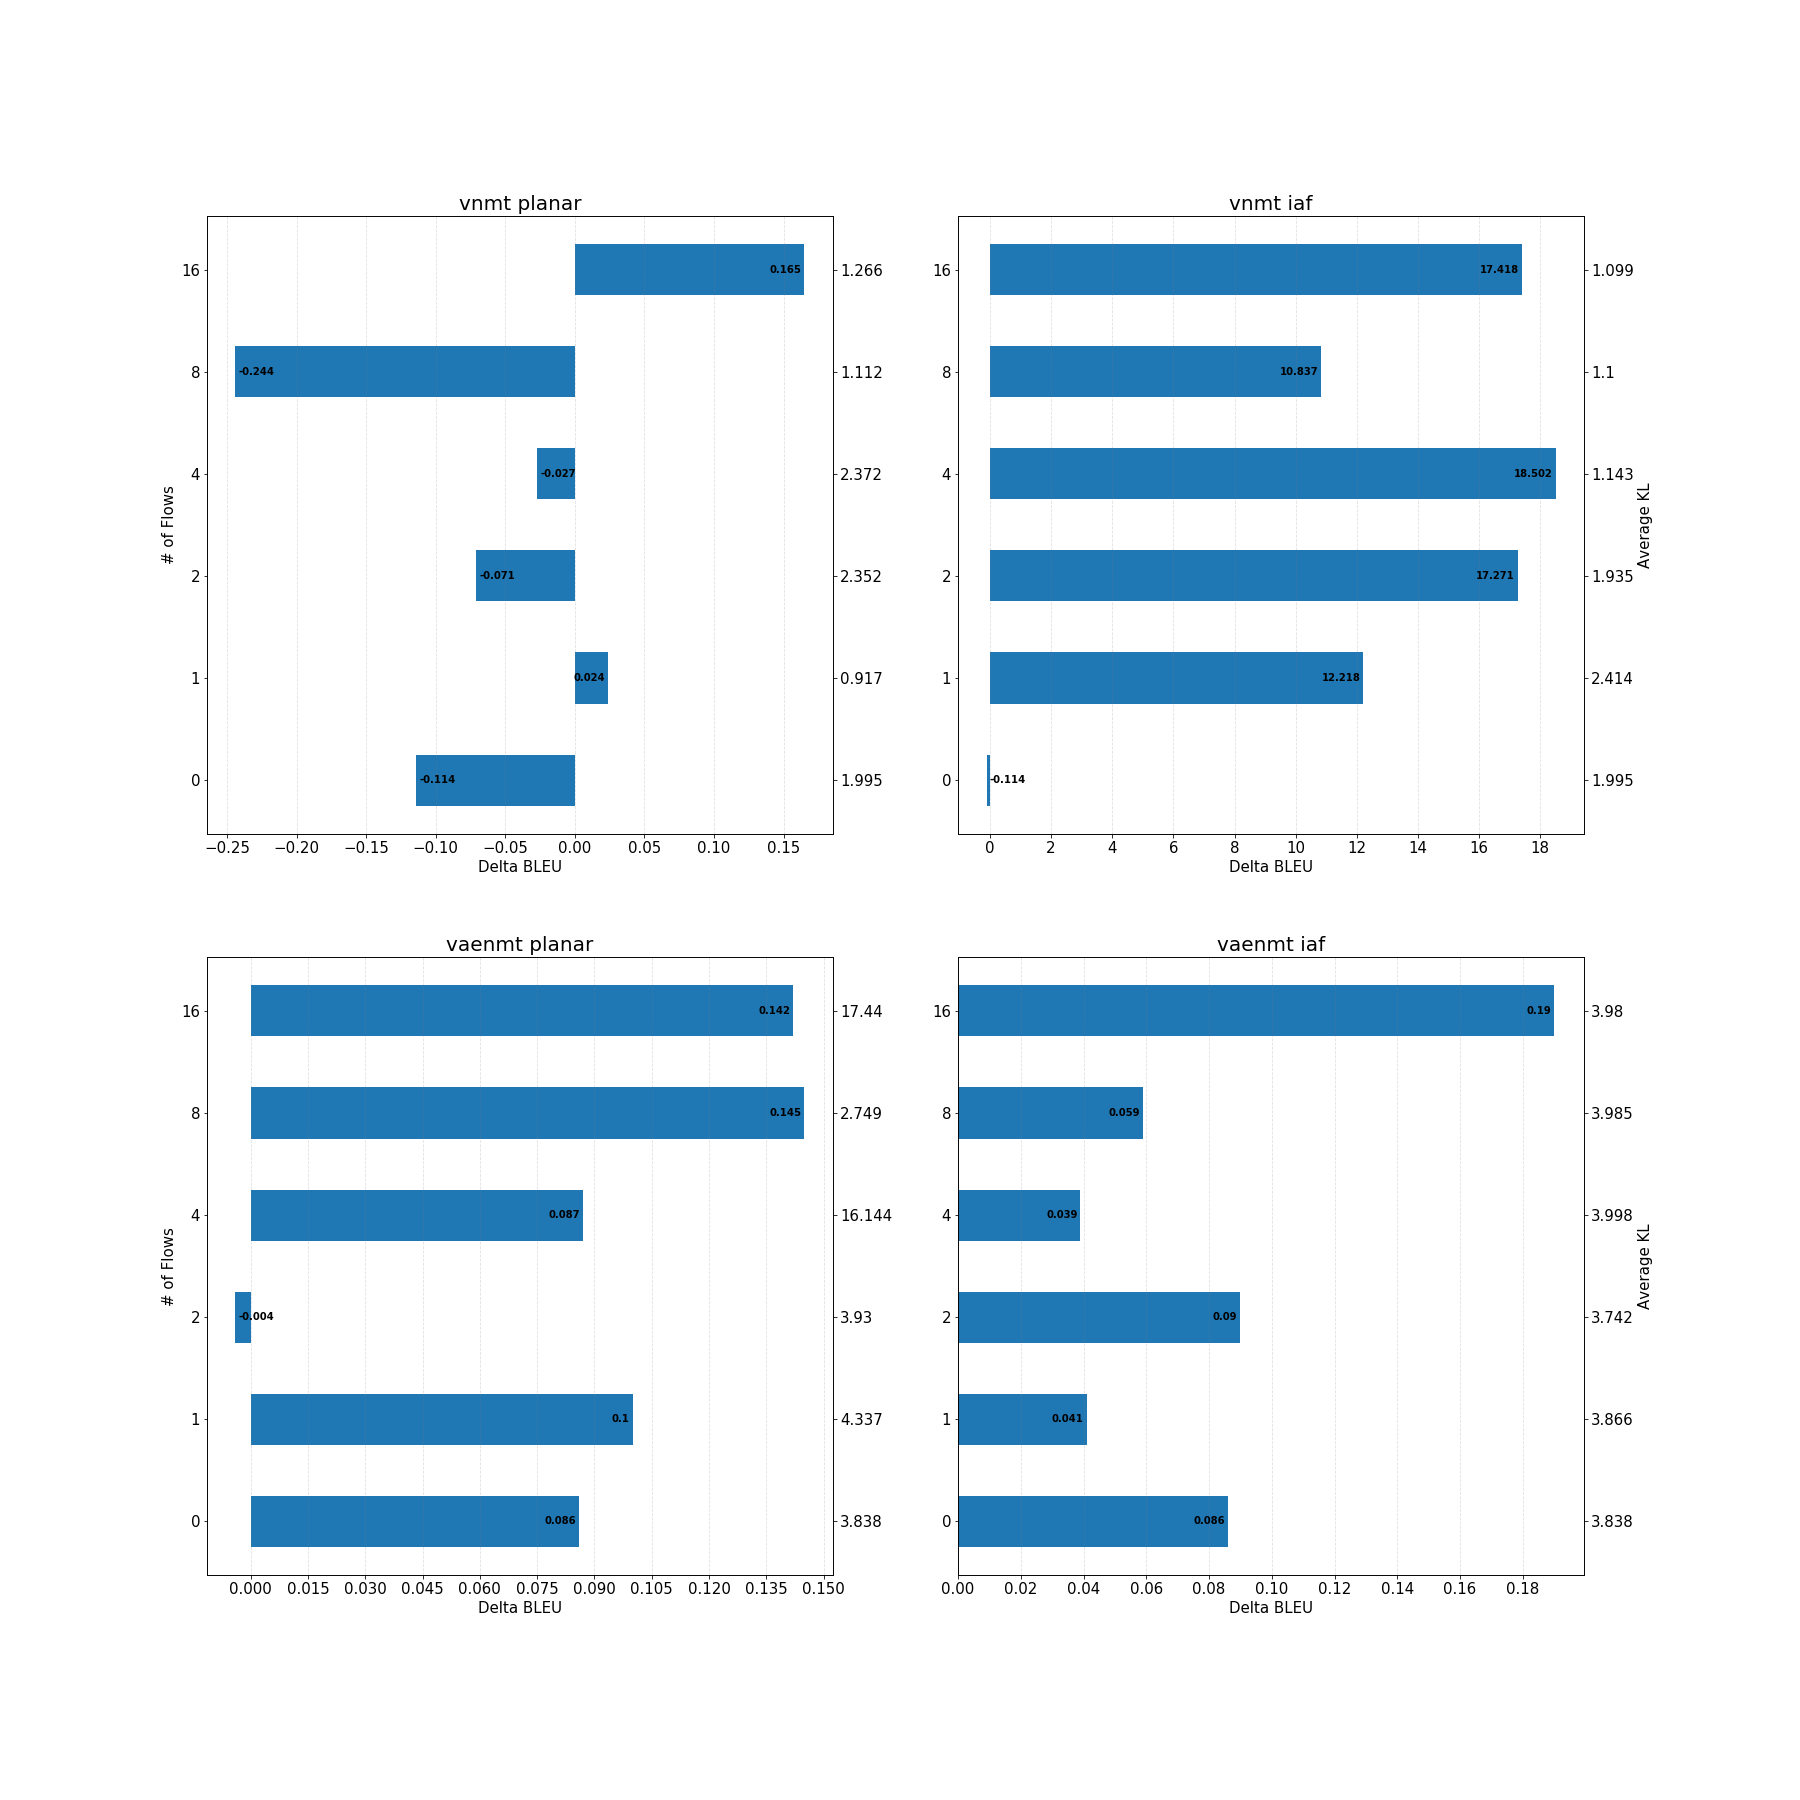
\includegraphics[width=\linewidth]{diff-z-256-horizontalbarplt.png}
%	\caption{The drop in performance when we set the value of the latent variable of Z to 0 during evaluation for latent dimensions set to 256. Bars are $BLEU_{Z=\mu} - BLEU_{Z=0}$. KL divergence of model is included on right axis, number of flows on left axis.}
%	\label{fig:barperfdrop}
%\end{figure}

\section{Language Modelling Performance}

%Hypothesis: Including normalizing flows improve the performance of the language model learned as part of the generative machine translation system. [This is related to a SPECIFIC model and is not applicable to the discriminative version of this stuff...just want to make sure that's clear]
For most of our previous experiments, we have found that \ac{GNMT} largely shows only slight gains from normalizing flows. As previously discussed in chapter 3, \ac{GNMT} trains a language model as part of the system.  In this section, we train \ac{GNMT} models that do not optimize this language model as part of the training procedure. The goal of this experiment is to test the impact of normalizing flows in the absence of language model for \ac{GNMT}.

Table \ref{tab:de_en_vaenmt_bleu_no_lm} shows our results with attention but no language model (in blue) compared against our \ac{GNMT} results from Table~\ref{tab:de_en_besttranslations}. Our results show similar performance to training our \ac{GNMT} model with the language model. At a 128 dimensional latent space our baseline still outperforms all flow models, as well as the training of \ac{GNMT} with a language model. At a 256 latent dimensional space, we see results close to our language model training, but with slight decreases in performance. Given how close these numbers are, these results suggest that $z$ is not the key factor for performance gains in our translation system for \ac{GNMT}. In addition, when we measure the KL divergence (see Table \ref{tab:de_en_vaenmt_bleu_no_lm_kl_divergence} ) we find that the latent variable has largely collapsed to the prior in many cases. Measurements of change of BLEU and without BLEU are in supplementary material Tables~\ref{tab:de_en_kl_divergence_sup}, \ref{tab:de_en_delta_bleu_sup},and  \ref{tab:de_en_vaenmt_bleu_no_lm_delta_bleu_sup}  as these show largely the same behaviour. 

Table \ref{tab:no_attn_no_lm_bleu} shows results of \ac{GNMT} with no language model training along with attention removed.  Here, we see that our flow models show some improvement over baselines unlike the \ac{GNMT} case. The language modelling seems to be more important as \ac{GNMT} does outperform our \ac{GNMT} without language modelling in several cases. Overall though, our best performances in this table is \ac{GNMT} without language modelling and a single planar flow. We did observe \textit{posterior collapse} (included in supplementary material) which might suggest these gains are not directly because of latent variable $z$. This could be simply a by-product of the stochastic behavior due to the training procedure. It has been previously suggested that the stochastic behaviour injected by latent variables does help with training performance \cite{Zhang2016VNMT}. 



\begin{table}[]
	\caption{BLEU scores for \ac{GNMT} without language model training. Bold entries are the best performing models. We include previous \ac{GNMT} results in red to compare with \ac{GNMT} without language model training (blue).}
	\label{tab:de_en_vaenmt_bleu_no_lm}	
	\center
	\begin{tabular}{cccccccc}
		\multicolumn{8}{c}{\textbf{Latent Dimension: 128}}                                                                                                                                                                                                                                                                                                                                                                                                                                                                                                \\ \hline
		\multicolumn{1}{|c|}{\textbf{Flows}}                          & \multicolumn{1}{c|}{\textbf{1}}                             & \multicolumn{1}{c|}{\textbf{2}}                             & \multicolumn{1}{c|}{\textbf{4}}                             & \multicolumn{1}{c|}{\textbf{8}}                    & \multicolumn{1}{c|}{\textbf{16}}                            & \multicolumn{1}{c|}{\textbf{0 (Baseline)}}                                    & \multicolumn{1}{c|}{\textbf{Model}}                                                  \\ \hline
		\rowcolor[HTML]{CEF2F1} 
		\multicolumn{1}{|c|}{\cellcolor[HTML]{CEF2F1}Planar}          & \multicolumn{1}{c|}{\cellcolor[HTML]{CEF2F1}20.46}          & \multicolumn{1}{c|}{\cellcolor[HTML]{CEF2F1}20.42}          & \multicolumn{1}{c|}{\cellcolor[HTML]{CEF2F1}20.5}           & \multicolumn{1}{c|}{\cellcolor[HTML]{CEF2F1}20.65} & \multicolumn{1}{c|}{\cellcolor[HTML]{CEF2F1}20.41}          & \multicolumn{1}{c|}{\cellcolor[HTML]{CEF2F1}}                                 & \multicolumn{1}{c|}{\cellcolor[HTML]{CEF2F1}}                                        \\ \cline{1-6}
		\rowcolor[HTML]{CEF2F1} 
		\multicolumn{1}{|c|}{\cellcolor[HTML]{CEF2F1}IAF}             & \multicolumn{1}{c|}{\cellcolor[HTML]{CEF2F1}20.48}          & \multicolumn{1}{c|}{\cellcolor[HTML]{CEF2F1}20.45}          & \multicolumn{1}{c|}{\cellcolor[HTML]{CEF2F1}20.71}          & \multicolumn{1}{c|}{\cellcolor[HTML]{CEF2F1}20.45} & \multicolumn{1}{c|}{\cellcolor[HTML]{CEF2F1}20.38}          & \multicolumn{1}{c|}{\multirow{-2}{*}{\cellcolor[HTML]{CEF2F1}\textbf{20.77}}} & \multicolumn{1}{c|}{\multirow{-2}{*}{\cellcolor[HTML]{CEF2F1}GNMT (No LM)}}          \\ \hline
		\rowcolor[HTML]{F4DAD8} 
		\multicolumn{1}{|c|}{\cellcolor[HTML]{F4DAD8}Planar}          & \multicolumn{1}{c|}{\cellcolor[HTML]{F4DAD8}20.59}          & \multicolumn{1}{c|}{\cellcolor[HTML]{F4DAD8}20.60}          & \multicolumn{1}{c|}{\cellcolor[HTML]{F4DAD8}20.48}          & \multicolumn{1}{c|}{\cellcolor[HTML]{F4DAD8}20.55} & \multicolumn{1}{c|}{\cellcolor[HTML]{F4DAD8}20.66}          & \multicolumn{1}{c|}{\cellcolor[HTML]{F4DAD8}}                                 & \multicolumn{1}{c|}{\cellcolor[HTML]{F4DAD8}}                                        \\ \cline{1-6}
		\rowcolor[HTML]{F4DAD8} 
		\multicolumn{1}{|c|}{\cellcolor[HTML]{F4DAD8}IAF}             & \multicolumn{1}{c|}{\cellcolor[HTML]{F4DAD8}20.64}          & \multicolumn{1}{c|}{\cellcolor[HTML]{F4DAD8}20.64}          & \multicolumn{1}{c|}{\cellcolor[HTML]{F4DAD8}20.51}          & \multicolumn{1}{c|}{\cellcolor[HTML]{F4DAD8}20.65} & \multicolumn{1}{c|}{\cellcolor[HTML]{F4DAD8}20.50}          & \multicolumn{1}{c|}{\multirow{-2}{*}{\cellcolor[HTML]{F4DAD8}\textbf{20.73}}} & \multicolumn{1}{c|}{\multirow{-2}{*}{\cellcolor[HTML]{F4DAD8}GNMT}}                  \\ \hline
		\multicolumn{8}{c}{\textbf{Latent Dimension: 256}}                                                                                                                                                                                                                                                                                                                                                                                                                                                                                                \\ \hline
		\multicolumn{1}{|c|}{\textbf{Flows}}                          & \multicolumn{1}{c|}{\textbf{1}}                             & \multicolumn{1}{c|}{\textbf{2}}                             & \multicolumn{1}{c|}{\textbf{4}}                             & \multicolumn{1}{c|}{\textbf{8}}                    & \multicolumn{1}{c|}{\textbf{16}}                            & \multicolumn{1}{c|}{\textbf{0 (Baseline)}}                                    & \multicolumn{1}{c|}{\textbf{Model}}                                                  \\ \hline
		\rowcolor[HTML]{CEF2F1} 
		\multicolumn{1}{|c|}{\cellcolor[HTML]{CEF2F1}Planar} & \multicolumn{1}{c|}{\cellcolor[HTML]{CEF2F1}20.32}          & \multicolumn{1}{c|}{\cellcolor[HTML]{CEF2F1}20.36}          & \multicolumn{1}{c|}{\cellcolor[HTML]{CEF2F1}20.47}          & \multicolumn{1}{c|}{\cellcolor[HTML]{CEF2F1}20.21} & \multicolumn{1}{c|}{\cellcolor[HTML]{CEF2F1}\textbf{20.65}} & \multicolumn{1}{c|}{\cellcolor[HTML]{CEF2F1}}                                 & \multicolumn{1}{c|}{\cellcolor[HTML]{CEF2F1}}                                        \\ \cline{1-6}
		\rowcolor[HTML]{CEF2F1} 
		\multicolumn{1}{|c|}{\cellcolor[HTML]{CEF2F1}IAF}    & \multicolumn{1}{c|}{\cellcolor[HTML]{CEF2F1}20.56}          & \multicolumn{1}{c|}{\cellcolor[HTML]{CEF2F1}\textbf{20.64}} & \multicolumn{1}{c|}{\cellcolor[HTML]{CEF2F1}20.51}          & \multicolumn{1}{c|}{\cellcolor[HTML]{CEF2F1}20.54} & \multicolumn{1}{c|}{\cellcolor[HTML]{CEF2F1}20.41}          & \multicolumn{1}{c|}{\multirow{-2}{*}{\cellcolor[HTML]{CEF2F1}20.59}}          & \multicolumn{1}{c|}{\multirow{-2}{*}{\cellcolor[HTML]{CEF2F1}GNMT (No LM)}} \\ \hline
		\rowcolor[HTML]{F4DAD8} 
		\multicolumn{1}{|c|}{\cellcolor[HTML]{F4DAD8}Planar}          & \multicolumn{1}{c|}{\cellcolor[HTML]{F4DAD8}20.55}          & \multicolumn{1}{c|}{\cellcolor[HTML]{F4DAD8}\textbf{20.67}} & \multicolumn{1}{c|}{\cellcolor[HTML]{F4DAD8}20.54}          & \multicolumn{1}{c|}{\cellcolor[HTML]{F4DAD8}20.51} & \multicolumn{1}{c|}{\cellcolor[HTML]{F4DAD8}\textbf{20.67}} & \multicolumn{1}{c|}{\cellcolor[HTML]{F4DAD8}}                                 & \multicolumn{1}{c|}{\cellcolor[HTML]{F4DAD8}}                                        \\ \cline{1-6}
		\rowcolor[HTML]{F4DAD8} 
		\multicolumn{1}{|c|}{\cellcolor[HTML]{F4DAD8}IAF}             & \multicolumn{1}{c|}{\cellcolor[HTML]{F4DAD8}20.85}          & \multicolumn{1}{c|}{\cellcolor[HTML]{F4DAD8}\textbf{20.86}} & \multicolumn{1}{c|}{\cellcolor[HTML]{F4DAD8}20.64}          & \multicolumn{1}{c|}{\cellcolor[HTML]{F4DAD8}20.62} & \multicolumn{1}{c|}{\cellcolor[HTML]{F4DAD8}20.66}          & \multicolumn{1}{c|}{\multirow{-2}{*}{\cellcolor[HTML]{F4DAD8}20.66}}          & \multicolumn{1}{c|}{\multirow{-2}{*}{\cellcolor[HTML]{F4DAD8}GNMT}}                  \\ \hline
	\end{tabular}
\end{table}


\begin{table}[]
	\caption{ \ac{GNMT} training results without attention or language model training. In several instances, \ac{GNMT} without language model training outperform models which optimize the language model. }
	\label{tab:no_attn_no_lm_bleu}
	\center
	\begin{tabular}{cccccccc}
		\multicolumn{8}{c}{\textbf{Latent Dimension: 128}}                                                                                                                                                                                                                                                                                                                                                                                                                                                            \\ \hline
		\multicolumn{1}{|c|}{\textbf{Flows}}                       & \multicolumn{1}{c|}{\textbf{1}}                            & \multicolumn{1}{c|}{\textbf{2}}                   & \multicolumn{1}{c|}{\textbf{4}}                   & \multicolumn{1}{c|}{\textbf{8}}                   & \multicolumn{1}{c|}{\textbf{16}}                           & \multicolumn{1}{c|}{\textbf{0 (Baseline)}}                                   & \multicolumn{1}{c|}{\textbf{Model}}                                         \\ \hline
		\rowcolor[HTML]{CEF2F1} 
		\multicolumn{1}{|c|}{\cellcolor[HTML]{CEF2F1}Planar}       & \multicolumn{1}{c|}{\cellcolor[HTML]{CEF2F1}7.23}          & \multicolumn{1}{c|}{\cellcolor[HTML]{CEF2F1}7.03} & \multicolumn{1}{c|}{\cellcolor[HTML]{CEF2F1}7.25} & \multicolumn{1}{c|}{\cellcolor[HTML]{CEF2F1}\textbf{7.32}} & \multicolumn{1}{c|}{\cellcolor[HTML]{CEF2F1}7.27}          & \multicolumn{1}{c|}{\cellcolor[HTML]{CEF2F1}}                                & \multicolumn{1}{c|}{\cellcolor[HTML]{CEF2F1}}                               \\ \cline{1-6}
		\rowcolor[HTML]{CEF2F1} 
		\multicolumn{1}{|c|}{\cellcolor[HTML]{CEF2F1}IAF}          & \multicolumn{1}{c|}{\cellcolor[HTML]{CEF2F1}\textbf{7.5}}  & \multicolumn{1}{c|}{\cellcolor[HTML]{CEF2F1}7.42} & \multicolumn{1}{c|}{\cellcolor[HTML]{CEF2F1}7.37} & \multicolumn{1}{c|}{\cellcolor[HTML]{CEF2F1}7.31} & \multicolumn{1}{c|}{\cellcolor[HTML]{CEF2F1}7.16}          & \multicolumn{1}{c|}{\multirow{-2}{*}{\cellcolor[HTML]{CEF2F1}7.31}}          & \multicolumn{1}{c|}{\multirow{-2}{*}{\cellcolor[HTML]{CEF2F1}GNMT (No LM)}} \\ \hline
		\rowcolor[HTML]{F4DAD8} 
		\multicolumn{1}{|c|}{\cellcolor[HTML]{F4DAD8}Planar}       & \multicolumn{1}{c|}{\cellcolor[HTML]{F4DAD8}7.2}           & \multicolumn{1}{c|}{\cellcolor[HTML]{F4DAD8}7.22} & \multicolumn{1}{c|}{\cellcolor[HTML]{F4DAD8}7.19} & \multicolumn{1}{c|}{\cellcolor[HTML]{F4DAD8}7.11} & \multicolumn{1}{c|}{\cellcolor[HTML]{F4DAD8}7.25}          & \multicolumn{1}{c|}{\cellcolor[HTML]{F4DAD8}\textbf{7.36}}                   & \multicolumn{1}{c|}{\cellcolor[HTML]{F4DAD8}}                               \\ \cline{1-7}
		\rowcolor[HTML]{F4DAD8} 
		\multicolumn{1}{|c|}{\cellcolor[HTML]{F4DAD8}IAF}          & \multicolumn{1}{c|}{\cellcolor[HTML]{F4DAD8}7.31}          & \multicolumn{1}{c|}{\cellcolor[HTML]{F4DAD8}7.37} & \multicolumn{1}{c|}{\cellcolor[HTML]{F4DAD8}7.33} & \multicolumn{1}{c|}{\cellcolor[HTML]{F4DAD8}7.18} & \multicolumn{1}{c|}{\cellcolor[HTML]{F4DAD8}\textbf{7.41}} & \multicolumn{1}{c|}{\cellcolor[HTML]{F4DAD8}7.36}                            & \multicolumn{1}{c|}{\multirow{-2}{*}{\cellcolor[HTML]{F4DAD8}GNMT}}         \\ \hline
		\multicolumn{8}{c}{\textbf{Latent Dimension: 256}}                                                                                                                                                                                                                                                                                                                                                                                                                                                            \\ \hline
		\multicolumn{1}{|c|}{\textbf{Flows}}                       & \multicolumn{1}{c|}{\textbf{1}}                            & \multicolumn{1}{c|}{\textbf{2}}                   & \multicolumn{1}{c|}{\textbf{4}}                   & \multicolumn{1}{c|}{\textbf{8}}                   & \multicolumn{1}{c|}{\textbf{16}}                           & \multicolumn{1}{c|}{\textbf{0 (Baseline)}}                                   & \multicolumn{1}{c|}{\textbf{Model}}                                         \\ \hline
		\rowcolor[HTML]{CEF2F1} 
		\multicolumn{1}{|c|}{\cellcolor[HTML]{CEF2F1}Planar}       & \multicolumn{1}{c|}{\cellcolor[HTML]{CEF2F1}\textbf{7.58}} & \multicolumn{1}{c|}{\cellcolor[HTML]{CEF2F1}7.45} & \multicolumn{1}{c|}{\cellcolor[HTML]{CEF2F1}7.28} & \multicolumn{1}{c|}{\cellcolor[HTML]{CEF2F1}7.44} & \multicolumn{1}{c|}{\cellcolor[HTML]{CEF2F1}7.33}          & \multicolumn{1}{c|}{\cellcolor[HTML]{CEF2F1}}                                & \multicolumn{1}{c|}{\cellcolor[HTML]{CEF2F1}}                               \\ \cline{1-6}
		\rowcolor[HTML]{CEF2F1} 
		\multicolumn{1}{|c|}{\cellcolor[HTML]{CEF2F1}IAF} & \multicolumn{1}{c|}{\cellcolor[HTML]{CEF2F1}7.25}          & \multicolumn{1}{c|}{\cellcolor[HTML]{CEF2F1}7.35} & \multicolumn{1}{c|}{\cellcolor[HTML]{CEF2F1}7.32} & \multicolumn{1}{c|}{\cellcolor[HTML]{CEF2F1}7.08} & \multicolumn{1}{c|}{\cellcolor[HTML]{CEF2F1}7.47}          & \multicolumn{1}{c|}{\multirow{-2}{*}{\cellcolor[HTML]{CEF2F1}7.21}}          & \multicolumn{1}{c|}{\multirow{-2}{*}{\cellcolor[HTML]{CEF2F1}GNMT (No LM)}} \\ \hline
		\rowcolor[HTML]{F4DAD8} 
		\multicolumn{1}{|c|}{\cellcolor[HTML]{F4DAD8}Planar}       & \multicolumn{1}{c|}{\cellcolor[HTML]{F4DAD8}7.4}           & \multicolumn{1}{c|}{\cellcolor[HTML]{F4DAD8}7.22} & \multicolumn{1}{c|}{\cellcolor[HTML]{F4DAD8}7.33} & \multicolumn{1}{c|}{\cellcolor[HTML]{F4DAD8}7.26} & \multicolumn{1}{c|}{\cellcolor[HTML]{F4DAD8}7.07}          & \multicolumn{1}{c|}{\cellcolor[HTML]{F4DAD8}}                                & \multicolumn{1}{c|}{\cellcolor[HTML]{F4DAD8}}                               \\ \cline{1-6}
		\rowcolor[HTML]{F4DAD8} 
		\multicolumn{1}{|c|}{\cellcolor[HTML]{F4DAD8}IAF}          & \multicolumn{1}{c|}{\cellcolor[HTML]{F4DAD8}7.35}          & \multicolumn{1}{c|}{\cellcolor[HTML]{F4DAD8}7.34} & \multicolumn{1}{c|}{\cellcolor[HTML]{F4DAD8}7.28} & \multicolumn{1}{c|}{\cellcolor[HTML]{F4DAD8}7.04} & \multicolumn{1}{c|}{\cellcolor[HTML]{F4DAD8}7.36}          & \multicolumn{1}{c|}{\multirow{-2}{*}{\cellcolor[HTML]{F4DAD8}\textbf{7.51}}} & \multicolumn{1}{c|}{\multirow{-2}{*}{\cellcolor[HTML]{F4DAD8}GNMT}}         \\ \hline
	\end{tabular}
\end{table}





\begin{table}[]
	\caption{KL divergence of \ac{GNMT} models without language model training. Typically a near 0 KL divergence with stationary priors indicates \textit{posterior collapse} has occurred.  }
	\label{tab:de_en_vaenmt_bleu_no_lm_kl_divergence}
	\center	
	\begin{tabular}{cccccccc}
		\multicolumn{8}{c}{\textbf{Latent Dimension: 128 (KL Divergence)}}                                                                                                                                                                                                                                                                                                                                                                                                                             \\ \hline
		\multicolumn{1}{|c|}{\textbf{Flows}}                          & \multicolumn{1}{c|}{\textbf{1}}                   & \multicolumn{1}{c|}{\textbf{2}}                   & \multicolumn{1}{c|}{\textbf{4}}                   & \multicolumn{1}{c|}{\textbf{8}}                   & \multicolumn{1}{c|}{\textbf{16}}                  & \multicolumn{1}{c|}{\textbf{0 (Baseline)}}                          & \multicolumn{1}{c|}{\textbf{Model}}                                                  \\ \hline
		\rowcolor[HTML]{CEF2F1} 
		\multicolumn{1}{|c|}{\cellcolor[HTML]{CEF2F1}Planar}          & \multicolumn{1}{c|}{\cellcolor[HTML]{CEF2F1}0.01} & \multicolumn{1}{c|}{\cellcolor[HTML]{CEF2F1}0.0}  & \multicolumn{1}{c|}{\cellcolor[HTML]{CEF2F1}0.0}  & \multicolumn{1}{c|}{\cellcolor[HTML]{CEF2F1}0.01} & \multicolumn{1}{c|}{\cellcolor[HTML]{CEF2F1}0.01} & \multicolumn{1}{c|}{\cellcolor[HTML]{CEF2F1}}                       & \multicolumn{1}{c|}{\cellcolor[HTML]{CEF2F1}}                                        \\ \cline{1-6}
		\rowcolor[HTML]{CEF2F1} 
		\multicolumn{1}{|c|}{\cellcolor[HTML]{CEF2F1}IAF}             & \multicolumn{1}{c|}{\cellcolor[HTML]{CEF2F1}0.0}  & \multicolumn{1}{c|}{\cellcolor[HTML]{CEF2F1}0.0}  & \multicolumn{1}{c|}{\cellcolor[HTML]{CEF2F1}0.0}  & \multicolumn{1}{c|}{\cellcolor[HTML]{CEF2F1}0.01} & \multicolumn{1}{c|}{\cellcolor[HTML]{CEF2F1}0.01} & \multicolumn{1}{c|}{\multirow{-2}{*}{\cellcolor[HTML]{CEF2F1}0.0}}  & \multicolumn{1}{c|}{\multirow{-2}{*}{\cellcolor[HTML]{CEF2F1}GNMT (No LM)}}          \\ \hline
		\rowcolor[HTML]{F4DAD8} 
		\multicolumn{1}{|c|}{\cellcolor[HTML]{F4DAD8}Planar}          & \multicolumn{1}{c|}{\cellcolor[HTML]{F4DAD8}3.23} & \multicolumn{1}{c|}{\cellcolor[HTML]{F4DAD8}3.15} & \multicolumn{1}{c|}{\cellcolor[HTML]{F4DAD8}2.36} & \multicolumn{1}{c|}{\cellcolor[HTML]{F4DAD8}2.82} & \multicolumn{1}{c|}{\cellcolor[HTML]{F4DAD8}3.64} & \multicolumn{1}{c|}{\cellcolor[HTML]{F4DAD8}}                       & \multicolumn{1}{c|}{\cellcolor[HTML]{F4DAD8}}                                        \\ \cline{1-6}
		\rowcolor[HTML]{F4DAD8} 
		\multicolumn{1}{|c|}{\cellcolor[HTML]{F4DAD8}IAF}             & \multicolumn{1}{c|}{\cellcolor[HTML]{F4DAD8}4.31} & \multicolumn{1}{c|}{\cellcolor[HTML]{F4DAD8}4.36} & \multicolumn{1}{c|}{\cellcolor[HTML]{F4DAD8}4.19} & \multicolumn{1}{c|}{\cellcolor[HTML]{F4DAD8}4.43} & \multicolumn{1}{c|}{\cellcolor[HTML]{F4DAD8}4.14} & \multicolumn{1}{c|}{\multirow{-2}{*}{\cellcolor[HTML]{F4DAD8}4.39}} & \multicolumn{1}{c|}{\multirow{-2}{*}{\cellcolor[HTML]{F4DAD8}GNMT}}                  \\ \hline
		\multicolumn{8}{c}{\textbf{Latent Dimension: 256  (KL Divergence)}}                                                                                                                                                                                                                                                                                                                                                                                                                            \\ \hline
		\multicolumn{1}{|c|}{\textbf{Flows}}                          & \multicolumn{1}{c|}{\textbf{1}}                   & \multicolumn{1}{c|}{\textbf{2}}                   & \multicolumn{1}{c|}{\textbf{4}}                   & \multicolumn{1}{c|}{\textbf{8}}                   & \multicolumn{1}{c|}{\textbf{16}}                  & \multicolumn{1}{c|}{\textbf{0 (Baseline)}}                          & \multicolumn{1}{c|}{\textbf{Model}}                                                  \\ \hline
		\rowcolor[HTML]{CEF2F1} 
		\multicolumn{1}{|c|}{\cellcolor[HTML]{CEF2F1}Planar} & \multicolumn{1}{c|}{\cellcolor[HTML]{CEF2F1}0.01} & \multicolumn{1}{c|}{\cellcolor[HTML]{CEF2F1}0.01} & \multicolumn{1}{c|}{\cellcolor[HTML]{CEF2F1}0.01} & \multicolumn{1}{c|}{\cellcolor[HTML]{CEF2F1}0.01} & \multicolumn{1}{c|}{\cellcolor[HTML]{CEF2F1}0.01} & \multicolumn{1}{c|}{\cellcolor[HTML]{CEF2F1}}                       & \multicolumn{1}{c|}{\cellcolor[HTML]{CEF2F1}}                                        \\ \cline{1-6}
		\rowcolor[HTML]{CEF2F1} 
		\multicolumn{1}{|c|}{\cellcolor[HTML]{CEF2F1}IAF}    & \multicolumn{1}{c|}{\cellcolor[HTML]{CEF2F1}0.0}  & \multicolumn{1}{c|}{\cellcolor[HTML]{CEF2F1}0.0}  & \multicolumn{1}{c|}{\cellcolor[HTML]{CEF2F1}0.0}  & \multicolumn{1}{c|}{\cellcolor[HTML]{CEF2F1}0.0}  & \multicolumn{1}{c|}{\cellcolor[HTML]{CEF2F1}0.01} & \multicolumn{1}{c|}{\multirow{-2}{*}{\cellcolor[HTML]{CEF2F1}0.0}}  & \multicolumn{1}{c|}{\multirow{-2}{*}{\cellcolor[HTML]{CEF2F1}GNMT (No LM)}} \\ \hline
		\rowcolor[HTML]{F4DAD8} 
		\multicolumn{1}{|c|}{\cellcolor[HTML]{F4DAD8}Planar}          & \multicolumn{1}{c|}{\cellcolor[HTML]{F4DAD8}4.34} & \multicolumn{1}{c|}{\cellcolor[HTML]{F4DAD8}3.93} & \multicolumn{1}{c|}{\cellcolor[HTML]{F4DAD8}3.36} & \multicolumn{1}{c|}{\cellcolor[HTML]{F4DAD8}2.75} & \multicolumn{1}{c|}{\cellcolor[HTML]{F4DAD8}3.62} & \multicolumn{1}{c|}{\cellcolor[HTML]{F4DAD8}}                       & \multicolumn{1}{c|}{\cellcolor[HTML]{F4DAD8}}                                        \\ \cline{1-6}
		\rowcolor[HTML]{F4DAD8} 
		\multicolumn{1}{|c|}{\cellcolor[HTML]{F4DAD8}IAF}             & \multicolumn{1}{c|}{\cellcolor[HTML]{F4DAD8}3.87} & \multicolumn{1}{c|}{\cellcolor[HTML]{F4DAD8}3.74} & \multicolumn{1}{c|}{\cellcolor[HTML]{F4DAD8}4.0}  & \multicolumn{1}{c|}{\cellcolor[HTML]{F4DAD8}3.99} & \multicolumn{1}{c|}{\cellcolor[HTML]{F4DAD8}3.98} & \multicolumn{1}{c|}{\multirow{-2}{*}{\cellcolor[HTML]{F4DAD8}3.84}} & \multicolumn{1}{c|}{\multirow{-2}{*}{\cellcolor[HTML]{F4DAD8}GNMT}}                  \\ \hline
	\end{tabular}
\end{table}





\chapter{Discussion}
\chapter{Conclusion}


%    3. Notes
%    4. Footnotes

%    5. Bibliography
\begin{singlespace}
\raggedright
\bibliographystyle{abbrvnat}
\bibliography{biblio}
\end{singlespace}

\appendix
%    6. Appendices (including copies of all required UBC Research
%       Ethics Board's Certificates of Approval)
%\include{reb-coa}	% pdfpages is useful here
\chapter{Supporting Materials}

This would be any supporting material not central to the dissertation.
For example:
\begin{itemize}
\item additional details of methodology and/or data;
\item diagrams of specialized equipment developed.;
\item copies of questionnaires and survey instruments.
\end{itemize}


\backmatter
%    7. Index
% See the makeindex package: the following page provides a quick overview
% <http://www.image.ufl.edu/help/latex/latex_indexes.shtml>


\end{document}
